% ----------------------------------------------------
% Magic Comments for LaTeX-editors (TeXstudio, VSCode with LaTeX Workshop extension...)
% !TeX encoding = utf8
% !TeX spellcheck = de_DE
% !TeX program = pdflatex
% !BIB program = biber
% ----------------------------------------------------

% ----------------------------------------------------
% Load the HfTL-Thesis class
\documentclass[
% Select the main Language of your thesis here. Titlepage, captions and statement of authorship will change accordingly:
%
% ngerman% - Deutsch (default)
% USenglish % - American english
% UKenglish % - British english
% numeric   % (default) use numeric citation style sorted by the occurence in text: [5]
% alphabetic % - use alphabetic citation style: [Lau95]
% authoryear % - use authoryear citation style: Laubach 1995
]{hftlthesis}
% ----------------------------------------------------

% ----------------------------------------------------
% Set your custom options here. See https://komascript.de/~mkohm/scrguide.pdf for possibilities.

%\KOMAoption{twoside}{true} % Enable double sided layout
%\KOMAoption{BCOR}{8.25mm} % Binding Correction, adds the specified margin to the inner side of the page (left on single sided layout). This is to compensate lost page margin due to binding.

% ----------------------------------------------------

% ----------------------------------------------------
% Load your own packages here
\usepackage{blindtext} % Only for demonstration purposes. Can be removed!
\usepackage{todonotes}
\usepackage{float}
\usepackage{tikz, pgfplots} % To create diagrams and figures directly with LaTeX
\usepackage{listings} % support for Sourcecodelistings. For more advanced, prettier highlighting use the minted package instead (https://github.com/gpoore/minted) -> Requires Python with Pygments installed.
\usepackage{siunitx} % provides support for SI unit handling
\usepackage[useregional]{datetime2} % support for formatted date
\usepackage{booktabs}
\usepackage{amssymb}
\usepackage{longtable}

% ----------------------------------------------------

% ----------------------------------------------------
% Variables for Titlepage, PDF properties...
% Below are the default values. Comment them out to change them!

%\university{Hochschule für Telekommunikation Leipzig (FH)}
%\institute{Institut für Telekommunikationsinformatik}
%\documentKind{Abschlussarbeit zur Erlangung des akademischen Grades}
%\forDegree{Bachelor of Engineering}
%
\topic{\enquote{Untersuchung des Stromverbrauchs von verschiedenen Algorithmen und deren Implementierung auf mobilen Geräten}}
%
\thesisAuthor{Niklas Kluge}
\authorDateOfBirth{27.06.1996}
\authorPlaceOfBirth{Wernigerode}
%
\handInDate{\DTMdate{2020-11-02}} %formatted custom date
%
\firstReviewerName{Prof. Dr. Ulf Schemmert}
\firstReviewerInstitution{Hochschule für Telekommunikation Leipzig}
\firstReviewerInstitutionStreet{Gustav-Freytag-Straße 43-45}
\firstReviewerInstitutionPlace{04277 Leipzig}
%
\secondReviewerName{Philipp Dockhorn, M. Eng.}
\secondReviewerInstitution{Hochschule für Telekommunikation Leipzig}
\secondReviewerInstitutionStreet{Gustav-Freytag-Straße 43-45}
\secondReviewerInstitutionPlace{04277 Leipzig}

% ----------------------------------------------------

% ----------------------------------------------------
% Include own references
\addbibresource{References/online.bib}
\addbibresource{References/3gpp.bib}
\addbibresource{References/etsi.bib}
\addbibresource{References/itut.bib}
%\addbibresource{References/rfc.bib}
\addbibresource{References/niklasLiteratur.bib}
% ----------------------------------------------------
% ----------------------------------------------------
% Set a list of directories, where graphics are stored, so you dont have to prepend the subdirectory in \includegraphics. The "Graphics" folder is set by default.

%\graphicspath{{./Graphics/}, {./Images}}
% ----------------------------------------------------

% ----------------------------------------------------
% Load acronym definitions
\input{acronyms}
\makenoidxglossaries % index acronyms

% ----------------------------------------------------

% ----------------------------------------------------
% The document body. Start your work here.
\begin{document}
\frontmatter % page numbers as small roman letters
\maketitle % print the titlepage
\cleardoublepage % start a new page

\chapter{Vorwort}
An dieser Stelle möchte ich mich bei Herr Dr. Schemmert für die zuverlässige Betreuung bedanken. Durch hilfreiche Ratschläge half mir Herr Schemmert bei der Findung zahlreicher Denkansätze, welche in der vorliegenden Arbeit Einzug erhalten haben. Des Weiteren möchte ich meiner Familie danken, die mir trotz familiärer Schicksalsschläge und gesundheitlicher Probleme während des Bearbeitungszeitraums genug Kraft geben konnte, um diese Arbeit rechtzeitig abzuschließen. % include the file Content/vorwort.tex
\cleardoublepage

\tableofcontents %print the table of contents
\cleardoublepage

\printnoidxglossary[type=\acronymtype] % print the list of abbreviations
\cleardoublepage

\listoffigures % print the list of figures
\cleardoublepage

\listoftables % print the list of tables
\cleardoublepage

\lstlistoflistings % print the list of source codes
\cleardoublepage	
	
\mainmatter %page numbers arabic, beginning from 1	

%Include the example document
%g% !TeX root = ../my-thesis.tex
\chapter{Beispiel zur Nutzung}
\section{Abkürzungen und Zitate}
Jedes Acronym hat einen Identifier, der komplett klein geschrieben wird. Im Beispiel: volte~-~nicht zu verwechseln mit der Abkürzung selbst (hier VoLTE). Im Abkürzungsverzeichnis werden alle Abkürzungen aufgelistet, mit allen Stellen, an denen sie Dokument verwendet wurden. 

\begin{minipage}{.6\textwidth}
\begin{lstlisting}[language=latex]
\ac{volte} % Erste Verwendung: 
% Langform (Abkürzung)
\ac{volte} % Zweite Verwendung: Abkürzung
\acs{isdn} % s = short: Abkürzung
\acl{ims} % l = long: Langform
\acf{iad} % f = full: Langform (Kurzform)
\end{lstlisting}   
\end{minipage}
\begin{minipage}{.4\textwidth}
	\footnotesize
	\textbf{Ergibt:}\\
	\ac{volte}\\
	\ac{volte}\\
	\acs{isdn}\\
	\acl{ims}\\
	\acf{iad} 
\end{minipage}

Bei der ersten Verwendung, wird die Langform ausgegeben, alle weitere Nutzungen der Abkürzung ergeben nur die Kurzform. Somit muss man nicht überlegen, ob die Abkürzung schon mal verwendet wurde, wie folgender Satz zeigt: 

\Ac{volte} ist eine tolle Erfindung \cite{3GPP.TS.24.228.v5.15.0}. Die Signalisierung läuft über das \ac{sip}~\cite{wikiNik}. \cite[S.~23]{fernandezgallardo_InstitutFurSoftwaretechnik_2017}
\cite[S.~50]{arnold2000java}

Auch das Zitieren von Quellen ist mit \LaTeX{} ein Kinderspiel! Treffe ich eine Aussage, so muss ich sie belegen~\cite{rfc2693}. Dies geschieht mit dem Befehl \lstinline[language=latex]|\cite{<bibid>}|. Mehrere Quellen werden durch eine kommagetrennte Liste an \texttt{BibIDs} im \texttt{cite} Befehl zitiert: \lstinline[language=latex]|\cite{<bibid1>, <bibid2>, <bibid2>}| ergibt: schrägstrich cite{rfc1, rfc1754, rfc1971}. Alle zitierten Quellen landen im Literaturverzeichnis.
\section{Bilder und Verweise}
\begin{figure}[ht]
	\centering
	\includegraphics[width=.85\linewidth]{turn-channeldata}
	\caption{Ein Vektografik Screenshot}
	\label{fig:turn-channeldata}
\end{figure}

Falls möglich sollten stets Vektorgrafiken verwendet werden. Diese können zum Beispiel mit Visio erstellt und als PDF exportiert werden. Die PDF Datei kann dann in \LaTeX{} als Grafik verwendet werden. Der Code hierfür lautet wie folgt:

% the float option prevents figures to be placed in the listing but also prevents the listing from spanning multiple pages
\begin{lstlisting}[language=latex,float]
\begin{figure}
	\centering %Zentrieren
	\includegraphics[width=.85\linewidth]{turn-channeldata} % Grafik einbinden (ohne Dateiendung) und auf 85 % der Seitenbreite Skalieren
	\caption{Ein Vektografik Screenshot} % Die Bildunterschrift
	\label{fig:turn-channeldata} % Das Label, mit dem die Grafik im Text referenziert werden kann
\end{figure}
\end{lstlisting}

Im Text kann ich auf eingebundene Abbildungen verweisen. In \autoref{fig:turn-channeldata} ist ein Vektorgrafik Screenshot zu sehen. Verwendet man \verb|\autoref{<label>}|, wird die Bezeichnung (Abbildung, Tabelle, Abschnitt\dots) automatisch ergänzt.


\begin{figure}[ht]
	\newcounter{density}
	\setcounter{density}{20}
	\centering
	\begin{tikzpicture}
	\def\couleur{cyan}
	\path[coordinate] (0,0)  coordinate(A)
	++( 90:5cm) coordinate(B)
	++(0:5cm) coordinate(C)
	++(-90:5cm) coordinate(D);
	\draw[fill=\couleur!\thedensity] (A) -- (B) -- (C) --(D) -- cycle;
	\foreach \x in {1,...,40}{%
		\pgfmathsetcounter{density}{\thedensity+20}
		\setcounter{density}{\thedensity}
		\path[coordinate] coordinate(X) at (A){};
		\path[coordinate] (A) -- (B) coordinate[pos=.10](A)
		-- (C) coordinate[pos=.10](B)
		-- (D) coordinate[pos=.10](C)
		-- (X) coordinate[pos=.10](D);
		\draw[fill=\couleur!\thedensity] (A)--(B)--(C)-- (D) -- cycle;
	}
	\end{tikzpicture}
	\caption{Rotated square from
		\href{http://www.texample.net/tikz/examples/rotated-polygons/}{texample.net}.}
	\label{fig:tikz1}
\end{figure}

Grafiken können auch direkt in \LaTeX{} mittles des TikZ Paketes erstellt werden (\autoref{fig:tikz1}). Auch verschiedenste Diagramme und Plots sind möglich (\autoref{fig:tikz2}). Zur vereinfachten Erstellung sind Tools, wie z.\,B. \href{https://www.mathcha.io}{https://www.mathcha.io} hilfreich.

\begin{figure}[ht]
	
	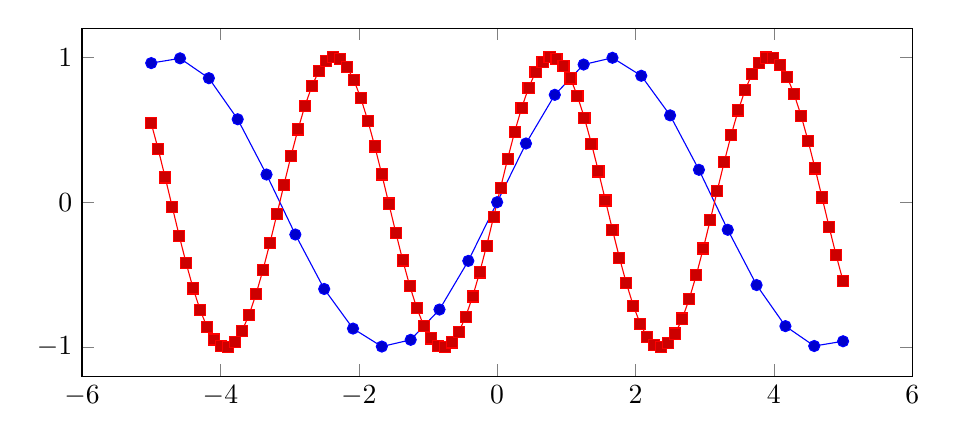
\begin{tikzpicture}
		\begin{axis}[
%		mlineplot,
		width=\textwidth,
		height=6cm,
		]
		
		\addplot {sin(deg(x))};
		\addplot+[samples=100] {sin(deg(2*x))};
		
		\end{axis}
	\end{tikzpicture}
	\caption{Ein Sinusplot mittels TiKZ}
	\label{fig:tikz2}
\end{figure}

\begin{figure}[ht]
	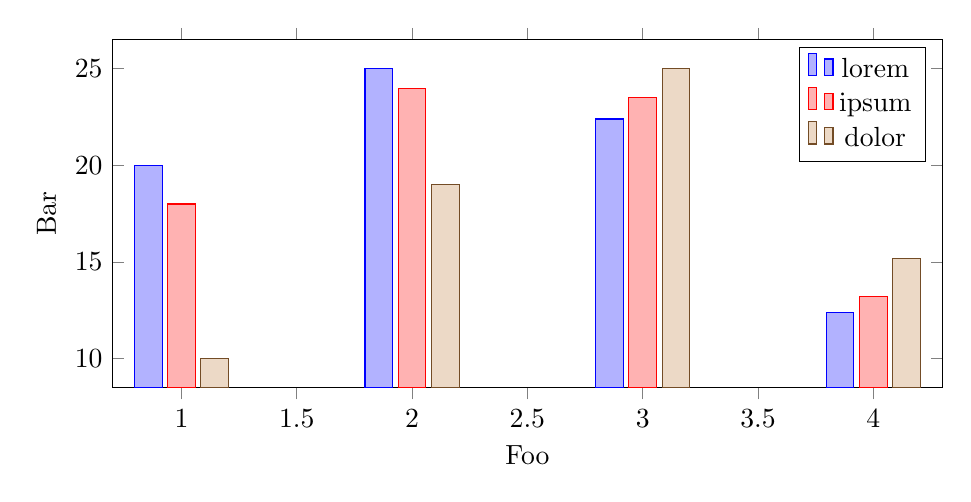
\begin{tikzpicture}
	\begin{axis}[
	ybar,
	xlabel={Foo},
	ylabel={Bar},
	width=\textwidth,
	height=6cm,
	]
	
	\addplot plot coordinates {(1, 20) (2, 25) (3, 22.4) (4, 12.4)};
	\addplot plot coordinates {(1, 18) (2, 24) (3, 23.5) (4, 13.2)};
	\addplot plot coordinates {(1, 10) (2, 19) (3, 25) (4, 15.2)};
	
	\legend{lorem, ipsum, dolor}
	
	\end{axis}
	\end{tikzpicture}
	\caption{Ein Balkendiagramm}
	\label{fig:tikz3}
\end{figure}

Wie in \autoref{fig:tikz3} zu sehen, sind auch Balkendiagramme möglich.

Mit \verb|\autoref{<label>}| kann man auch auf Abschnitte oder Kapitel verweisen. Im PDF wird automatisch eine Verlinkung hinzugefügt (siehe \autoref{sec:kommunikationsvorgange}).

\section{Tabellen}
\begin{otherlanguage*}{USenglish} % Switch document language temporarily but keep labels in main language. For better hyphenation! Use the unstarred variant to translate the labels as well.
\begin{table}
	\centering
	\caption[Modes of operation according to \glsentrytext{itu-t}]{Modes of operation according to \textcite{ITU-T.P.564}}
	\label{tab:modes_P.564}
	\begin{tabularx}{\textwidth}{@{}lclX@{}}
		\toprule
		\multicolumn{1}{c}{\textbf{Class}} & \textbf{Mode} & \multicolumn{1}{c}{\textbf{Name}} & \multicolumn{1}{c}{\textbf{Description}}                                                                            \\ \midrule
		\multirow{5}{*}{Midpoint}          & \multirow{2}{*}{A}             & \multirow{2}{*}{Dynamic operation}                 & The model uses information from RTCP-XR packets to optimize its prediction. \\ \cmidrule{2-4}
		& \multirow{2}{*}{B}             & \multirow{2}{*}{Static operation}                  & The model has been optimized or configured using \textit{a priori} knowledge of the endpoint.                                \\ \midrule
		\multirow{2}{*}{Endpoint}                            & \multirow{2}{*}{C}             & \multirow{2}{*}{Embedded operation}                & The model is co-located with the jitter buffer in the endpoint and has access to the jitter buffer.                 \\ \bottomrule
	\end{tabularx}

\end{table}
\end{otherlanguage*}
Tabellen können kompliziert in der Erstellung sein. Zum Glück gibt es Hilfsmittel wie den \enquote{\LaTeX{} Tables Generator}~\footnote{\href{https://www.tablesgenerator.com/}{https://www.tablesgenerator.com/}}. Dann ist auch die Erstellung von komplexeren Layouts wie in \autoref{tab:modes_P.564} kein Problem.


\section{Quellcode}
Auch Quellcode mit automatischem Syntaxhighlighting kann eingebunden werden. Die Referenzierung funktioniert auch hier (siehe \autoref{lst:signalexample}). Für noch schönere Quellcodelistings empfiehlt sich das Paket \href{https://ctan.org/pkg/minted?lang=de}{\texttt{minted}}, welches anstelle des \texttt{listings} Paket verwendet wird (Python benötigt!).
\begin{lstlisting}[language=c,caption={[Ein einfaches Quellcodelisting]Ein einfaches Quellcodelisting~\cite{wolf_LinuxsystemprogrammierenCKurs_2003}},label=lst:signalexample]
#include <stdio.h>
#include <stdlib.h>
#include <signal.h>

void sigfunc(int sig) {
	char c;
	if(sig != SIGINT)
		return;
	else {
		printf("\nWollen sie das Programm beenden (j/n) : ");
		c=getchar();
		if(c=='j')
			exit(0);
		return;
	}
}
int main() {
	int i;
	signal(SIGINT,sigfunc);
	while(1) {
	printf("Die Endlosschleife können sie mit STRG-C beenden");
	for(i=0;i<48;i++) {
		printf("\b"); //Cursor nach links bewegen
	}
	return 0;
}
\end{lstlisting}

\section{Sonstiges}
Es wird auch eine Umgebung für Beschreibungen bereitgestellt, bei denen das Label rechtsbündig ausgerichtet ist und die Beschreibung linksbündig. In die eckigen Klammern kommt das längste Label, damit \LaTeX{} die Abstände automatisch berechnen kann. Im Folgenden wird ein Beispiel für so eine Umgebung gebracht:

\begin{lstlisting}[language=latex,breaklines]
\begin{aligneddescription}[Registration success rate]
	\item[Registration success rate] describes the rate of successful registration attempts with the \ac{webrtc} signaling server.
	\item[Service availability] is defined in terms of capacity to establish calls from, and to \ac{webrtc} endpoints. 
	\item[Post dialing delay] is the time interval (in seconds) between the end of dialing by the caller and the reception back by him of the appropriate ringing tone or recorded announcement.
	\item[Call drop rate] equals service continuity in terms of capacity to maintain calls to their normal end.
\end{aligneddescription}
\end{lstlisting}
Das Ergebnis sieht wie folgt aus:
\begin{otherlanguage*}{USenglish} % switch to english hyphenation again
\begin{aligneddescription}[Registration success rate]
	\item[Registration success rate] describes the rate of successful registration attempts with the \ac{webrtc} signaling server.
	\item[Service availability] is defined in terms of capacity to establish calls from, and to \ac{webrtc} endpoints. 
	\item[Post dialing delay] is the time interval (in seconds) between the end of dialing by the caller and the reception back by him of the appropriate ringing tone or recorded announcement.
	\item[Call drop rate] equals service continuity in terms of capacity to maintain calls to their normal end.
\end{aligneddescription}
\end{otherlanguage*}

Des Weiteren bietet \KOMAScript{} die \texttt{labeling} Umgebung. Diese arbeitet ähnlich wie die \texttt{aligneddesription} Umgebung, jedoch sind die Labels linksbündig ausgerichtet. Das Ergebnis sieht wie folgt aus:

\begin{otherlanguage*}{USenglish} % switch to english hyphenation again
\begin{labeling}{Registration success rate}
	\item[Registration success rate] describes the rate of successful registration attempts with the \ac{webrtc} signaling server.
	\item[Service availability] is defined in terms of capacity to establish calls from, and to \ac{webrtc} endpoints. 
	\item[Post dialing delay] is the time interval (in seconds) between the end of dialing by the caller and the reception back by him of the appropriate ringing tone or recorded announcement.
	\item[Call drop rate] equals service continuity in terms of capacity to maintain calls to their normal end.
\end{labeling}
\end{otherlanguage*}

Hier zum Vergleich die Standard \texttt{description} Umgebung:

\begin{otherlanguage*}{USenglish} % switch to english hyphenation again
\begin{description}
	\item[Registration success rate] describes the rate of successful registration attempts with the \ac{webrtc} signaling server.
	\item[Service availability] is defined in terms of capacity to establish calls from, and to \ac{webrtc} endpoints. 
	\item[Post dialing delay] is the time interval (in seconds) between the end of dialing by the caller and the reception back by him of the appropriate ringing tone or recorded announcement.
	\item[Call drop rate] equals service continuity in terms of capacity to maintain calls to their normal end.
\end{description}
\end{otherlanguage*}

\section{Mathematik}
Auch mathematische Gleichungen können verwendet werden. In \autoref{eq:pam} ist ein Beispiel unter Verwendung der \texttt{equation} in Kombination mit der \texttt{split} Umgebung zu sehen. Damit können lange Gleichungen an bestimmten stellen umgebrochen und ausgerichtet werden.

\begin{equation}\label{eq:pam}
\begin{split}
f_{PAM_{M}}(t) = A_{T}\cdot \dfrac{T_{i}}{T_{T}} \Bigg[ 1+& \dfrac{A_{M}}{A_{T}}\cdot \mathrm{si}\left(f_{M}\cdot T_{i}\cdot \pi \right) \cdot \cos{\omega_{M}t} + \\
& \sum _{n=1}^{\infty }2\cdot \mathrm{si}\left(n\cdot f_{T}\cdot T_{i} \cdot \pi \right)\cos{\left(n\cdot \omega_{T} t \right)}  +  \\
& \sum _{n=1}^{\infty } \dfrac{A_{M}}{A_{T}} \cdot \mathrm{si}\left((n\cdot f_{T} + f_{M}) \cdot T_{i} \cdot \pi \right)\cos{\left(n\cdot \omega_{T} + \omega_{M}\right)}t +  \\
& \sum _{n=1}^{\infty } \dfrac{A_{M}}{A_{T}} \cdot \mathrm{si}\left((n\cdot f_{T} - f_{M})\cdot T_{i} \cdot \pi \right)\cos{\left(n\cdot \omega_{T} - \omega_{M})t\right)} \Bigg]
\end{split}
\end{equation}

Auch Gleichungen können mit einem Label versehen werden und mittels \lstinline[language=latex]|\autoref{<label>}| im Text referenziert werden. Siehe \autoref{eq:snr}. Der nachfolgende Code ergibt \autoref{eq:snr} und kann mittels \lstinline[language=latex]|\autoref{eq:snr}| referenziert werden:

\begin{lstlisting}[language=latex,breaklines]
\begin{equation}\label{eq:snr}
SNR(\si{\decibel}) = 10 \cdot \log_{10}\Bigg(\dfrac{P_{S}}{P_{R}} \Bigg)
\end{equation}
\end{lstlisting}

\begin{equation}\label{eq:snr}
	SNR(\si{\decibel}) = 10 \cdot \log_{10}\Bigg(\dfrac{P_{S}}{P_{R}} \Bigg)
\end{equation}

Auch der Umgang mit Einheiten ist dank des \texttt{siunitx} Paketes sehr einfach. So wird beispielsweise aus \lstinline[language=latex]|\SI{24.06}{\kilo\bit\per\second}|: \SI{24.06}{\kilo\bit\per\second} und aus \lstinline[language=latex]|\SIrange{20} {20000}{\hertz}|: \SIrange{20}{20000}{\hertz}.

% Include the other chapters
% !TeX root = ../my-thesis.tex
\chapter{Einleitung}
\section{Thematische Einführung}
Mobile Gräte wie Smartphones oder Tablets sind aus dem heutigen Alltag der Menschen nicht mehr wegzudenken. Ob zur privaten Unterhaltung beim spielen aufwendiger 3D Spiele, streamen von Musik- und Videoinhalten oder als unentbehrliches Werkzeug bei der täglichen Arbeit, mobile Geräte sind nahezu den gesamten Tag im Einsatz. Auch die Außendiensttechniker der DT Technik GmbH nutzen mobile Applikationen wie die Bestell-App oder die Mess-App zur Verwaltung und Aufstockung ihrer Werkzeuge und Ersatzteile beziehungsweise zur Untersuchung und Konfiguration von Routern. Hohe Akkulaufzeiten sind für diese Art der Benutzung eine Voraussetzung und stellen Smartphone Hersteller sowie Softwareentwickler vor die Herausforderung energieeffiziente Lösungen zu finden.
Dabei werden verschiedene Ansätze verfolgt. Auf der einen Seite versuchen die Hersteller energiesparende Prozessoren und Displays zu entwickeln und die Hardwarenutzung zu optimieren. Dieses Bestreben steht jedoch im Konflikt mit den Wünschen der Kunden, welche schnellere Mehrkern Prozessoren und größere Displays für die neuen Geräte erwarten. Dieser Trend ist auch in der Marktentwicklung der letzten zehn Jahre zu beobachten. So entsprach die durchschnittliche Displaygröße 2009 c.a. 3,2 Zoll. Acht Jahre später waren bereits Displays mit 5,5 Zoll üblich \cite{DisplayGroesse}. Auf der anderen Seite versuchen Anwendungsentwickler durch Softwareoptimierung ihre Applikationen ressourcensparender zu gestalten. Dabei können Prozesse wie zum Beispiel größere Downloads für Datenbankupdates als Service oder mithilfe des neuen Android Work Manager's als Hintergrundprozess implementiert werden und in Abhängigkeit vom aktuellen Ladestand des Akkus auf günstigere Zeitpunkte verschoben werden \cite{WorkManager}. Auch das gewissenhafte Umgehen mit Wake Locks und das festlegen der Standby Phasen der eigenen Applikation sind wichtige Stellschrauben, über welche ein Anwendungsentwickler energiesparende Anpassungen justieren kann \cite{WakeLocks}. Dies sind nur einige Beispiele  der möglichen Optionen für Energieoptimierungen auf mobilen Geräten. Das Problem der Energieeffizienz auf mobilen Geräten bietet ein breites Feld an Forschungspotential und wird auch zukünftig eine zentrale Rolle in der Geräteherstellung und App-Entwicklung spielen.

\section{Thematische Abgrenzung und Zielstellung dieser Arbeit}

In dieser Arbeit werden verschiedene Implementierungsansätze für Algorithmen und Berechnungen betrachtet und auf deren Einfluss hinsichtlich des Energieverbrauchs mobiler Geräte untersucht. Der Schwerpunkt liegt hierbei auf der Betrachtung von parallelen Berechnungen mithilfe von Multithreading. Dabei wird der Zusammenhang zwischen der Anzahl der parallel laufenden Threads, der Laufzeitveränderung und dem damit einhergehenden Energieverbrauch gemessen.
Ziel dieser Untersuchung ist es, herauszufinden ob es einen Zusammenhang zwischen den drei genannten Parametern gibt und gegebenenfalls eine Empfehlung für die Implementierung von Multithreading herauszuarbeiten, welche einen sinnvollen Kompromiss aus Laufzeit und Energieverbrauch bereitstellt.
Weiterhin wird der Unterschied zwischen rekursiven und iterativen Implementierungen hinsichtlich des Stromverbrauchs betrachtet. Auch hier ist das Ziel, die ressourcenschonendste Variante zu ermitteln.


\section{Struktureller Aufbau und Vorgehensweise der Untersuchung}

Das anschließende Kapitel \glqq Untersuchte Konzepte und Implementierungen\grqq{} beschreibt die theoretischen Aspekte von paralleler Programmierung und deren Einfluss auf den Energieverbrauch sowie die für diese Arbeit relevanten Gesetzmäßigkeiten und Berechnungsformeln des Multiprocessings. Außerdem werden die zur Untersuchung entwickelten Implementierungen vorgestellt, welche in der \glqq EnergyEfficience\grqq{} Applikation angewandt werden. Für die Umsetzung einer parallelen Ausführung wurde ein Base64 Encoder implementiert. Dieser ist nur ein Mittel zum Zweck und könnte durchaus durch andere lineare Algorithmen ersetzt werden. Des Weiteren werden auch die Unterschiede von rekursiven und iterativen Algorithmen beleuchtet und gegenübergestellt, da diese den zweiten großen Untersuchungsgegenstand dieser Arbeit bilden. Weil der Merge Sort Algorithmus aufgrund seiner Vielseitigkeit perfekt für die Gegenüberstellung dieser beiden Implementierungsstrategien geeignet ist, werden in diesem Kapitel die verwendeten Merge Sort Varianten inklusive ihrer Implementierung dargestellt.

Im folgenden Kapitel 3 \glqq Verwendete Geräte und Tools\grqq{} werden alle Programme und Geräte samt deren Spezifikationen vorgestellt, die im Rahmen dieser Untersuchung genutzt wurden. Es wird eine kurze Einführung in die Verwendung des Programms Battery Historian geben. Weiterhin wird die eigens für diese Arbeit entwickelte App vorgestellt. Anschließend wird die Messmethode mithilfe dieser beiden Tools beschrieben.

In Kapitel 4 \glqq Energieeffizientes Multithreading\grqq{} werden die Ergebnisse der Messungen des parallelen Base64 Encoders dargestellt und ausgewertet. Der Fokus liegt hierbei auf dem Zusammenhang zwischen verwendeter Thread-Anzahl und Energieverbrauch.

Daraufhin untersucht Kapitel 5 \glqq Rekursive und Iterative Verfahren im Vergleich\grqq{} den Einfluss von iterativer beziehungsweise rekursiver Implementierung auf den Energieverbrauch. Hierfür wird die bereits erwähnte Merge Sort Implementierung der \glqq EnergyEfficience\grqq{} Applikation genutzt. Außerdem werden die Vorzüge des Fork-Join Thread Pools bei paralleler Rekursion durch Messungen untersucht..

Im abschließenden Kapitel 6 \glqq Auswertung\grqq{} ist eine Zusammenfassung der gewonnen Erkenntnisse zu finden. Außerdem werden im Ausblick Ansätze für weitere Untersuchungen auf diesem Gebiet formuliert.


% !TeX root = ../my-thesis.tex
\chapter{Untersuchte Konzepte und Implementierungen}

\section{Theoretische Aspekte in die Parallelität}
Das Ziel hinter der Parallelisierung von Aufgaben ist die Beschleunigung der Laufzeit bei der Abarbeitung von Programmabläufen und die Minimierung der Wartezeiten des Prozessors. Solche Wartezeiten können entstehen, wenn während der Programmausführung Benutzereingaben nötig sind, bevor die Ausführung fortgesetzt werden kann oder wenn neue Daten aus dem vergleichsweise langsamen Hauptspeicher nachgeladen werden müssen, falls der prozessoreigene Cache nicht groß genug ist, um alle nötigen Daten für die aktuelle Ausführung auf einmal zu laden\cite[1135]{wolf2020}. Ohne Parallelität würden moderne Softwareanwendungen jeglicher Art nahezu unnutzbar werden. Einfache Vorgänge wie das Laden von Benutzerdaten aus einer lokalen Datenbank oder das Downloaden von Bildern aus dem Netz, würden ohne Parallelität beispielsweise zum Einfrieren der Benutzeroberfläche führen, da bei sequentiellen Programmabläufen alle Aufgaben strikt hintereinander ausgeführt werden müssen. Android selbst wäre ohne Parallelität nicht umsetzbar, da Androids Architektur Multithreading und damit Parallelität voraussetzt.

Für die Realisierung von Parallelität haben sich mit der Evolution der Prozessortechnologie verschieden Ansätze und Techniken entwickelt. Jede dieser Techniken ist bis heute relevant und glänzt in unterschiedlichen Anwendungsfällen.

\underline{Pipelining}

Beim Pipelining wird die Ausführung von Befehlen in verschiedene Phasen aufgeteilt, die jeweils durch eine eigene Ausführungseinheit bearbeitet werden. Sobald ein Befehl die aktuelle Phase abgeschlossen hat und zur nächsten Phase springt, kann bereits mit der Bearbeitung des nächsten Befehls in der frei gewordenen Phase begonnen werden. In \autoref{fig:Pipeline} ist ein Beispiel einer 5-Phasen Pipeline veranschaulicht. Die Bearbeitung jeder Phase dauert im Optimalfall einen Taktzyklus, da andernfalls die Pipeline bei der Bearbeitung der nachfolgenden Befehle in dieser Phase geblockt wird. Dies ist zum Beispiel in \autoref{fig:Pipeline} bei Befehl drei während der Execute Phase der Fall. Ein großer Nachteil von Pipelining tritt bei häufigen Programmsprüngen auf, da bei jedem Sprung die komplette Pipeline geleert werden muss und alle Phasen, die bis dorthin vollendet wurden, verworfen werden und umsonst bearbeitet wurden. Dieser Umstand ist besonders bei größeren Pipelines kritisch, da die einzelnen Befehle für längere Zeiträume in der Pipeline gehalten werden \cite{pipelineElektro}.
\begin{figure}[H]
	\begin{center}	 
	\includegraphics[scale=1]{Pipeline}
	\caption{Beispiel für eine 5-Phasen-Pipeline (Quelle: \cite{pipelineElektro})}
	\label{fig:Pipeline} 
	\end{center}
\end{figure}

\underline{simultanes Multithreading}

Ein Thread ist ein sequenzieller Ausführungspfaden innerhalb eines Prozesses, der ausgeführt wird. Bei Rechnern mit nur einem physischen Rechenkern kann zu einem Zeitpunkt immer nur ein Thread eines Prozesses gleichzeitig ausgeführt werden. Falls diese Ausführung durch Ereignisse wie Speicherzugriffe oder Nutzereingaben unterbrochen wird, blockiert der zugewiesene Thread die \ac{cpu} vollständig, sofern kein Multithreading betrieben wird. Durch sogenanntes simultanes Multithreading wird die verfügbare \ac{cpu} Rechenzeit auf mehrere Prozesse und Threads aufgeteilt. Die \ac{cpu} kann dadurch zwischen den Threads hin und her springen und so längere Wartezeiten verhindern. Dies steigert die Effizienz der \ac{cpu} hinsichtlich der Laufzeit sowie des Energieverbrauchs \cite[877]{cplusplus}. Diese Technik ermöglicht auch auf Systemen mit nur einem physischen Rechenkern den Eindruck von Parallelität und führt zu besser Nutzbarkeit der Anwendungen.

\underline{Hyperthreading}

Die Technologie Hyperthreading wurde von Intel mit den Prozessoren Pentium 3, Pentium 4 und Xeon eingeführt. Hierbei wird der Durchsatz von multithreaded Anwendungen im Multitasking erhöht, indem die Auslastung der On-Chip-Ressourcen erhöht wird, die in der Intel-NetBurst-Mikroarchitektur verfügbar sind. Ein typischer Thread belastet nur etwa 35 \% der NetBurst-Ausführungsressourcen. Hyperthreading erhöht die Auslastung durch notwendige Logik und Ressourcen, die der CPU hinzugefügt werden. Für die Aufteilung der reinkommenden Daten auf den freien Raum sorgen somit zwei logische Prozessoren, die vom Betriebssystem mittels klassischer Multiprocessing-Verfahren verwaltet werden \cite[1138]{wolf2020}. Somit stehen dem Rechner, trotz physischer Single-Core \ac{cpu}, daher zwei logische Rechenkerne zur Verfügung. Dies bietet die Möglichkeit Speicherwartezeit zu vermeiden, die ohne diese Technik die gesamte \ac{cpu} blockieren würde. Wenn der erste Thread im Wartezustand ist, kann der Prozessor mithilfe des zweiten logischen Kerns in der Programmausführung  der anderen Prozesse fortfahren.

\underline{Multicore-Prozessor}

Bei Multicore Systemen handelt es sich um Prozessoren mit mehreren physischen Rechenkernen. Diese können voneinander unabhängig arbeiten und ermöglichen echte Parallelität. Alle Rechenkerne nutzen zusätzlich die schon genannten Techniken, um möglichst effiziente Ergebnisse zu erhalten. Der Vorteil liegt hierbei nicht nur in der Steigerung der Geschwindigkeit. Mehrkernprozessoren können wesentlich geringer getaktet werden als Single-Core Prozessoren und ermöglichen trotzdem erhöhte Laufzeitgeschwindigkeit bei geringerer Leistungsaufnahme und Wärmeentwicklung \cite{MulicoreElektro}. Es könnte die Annahme getroffen werden, dass mit steigender Rechenkernzahl auch die Rechenleistung äquivalent ansteigt. Sodass die neue Laufzeit im Multi-Core-Betrieb gleich der ursprünglichen Laufzeit mit einem Kern geteilt durch die Anzahl der Rechenkerne ist. In der Realität ist dies jedoch nicht umsetzbar, da verschiedene Faktoren diese Annahme begrenzen. Zunächst einmal wächst mit steigender Anzahl an Rechenkernen auch der Aufwand der Verwaltung durch das Betriebssystem. Außerdem ist es nicht einfach den Zugriff auf geteilte Speicherressourcen durch mehrere Rechenkerne zu synchronisieren. Die Laufzeit für parallele Prozesse setzt sich grob aus folgenden Anteilen zusammen.
\begin{aligneddescription}
\item[Rechenzeit] Zeit für die Durchführung von Berechnungen unter Verwendung von Daten im lokalen Speicher der einzelnen Prozessoren.
\item[Kommunikationszeit] Zeit für den Austausch von Daten zwischen Prozessoren.
\item[Wartezeit] Z.B. aufgrund ungleicher Verteilung von Last zwischen den Rechenkernen, Datenabhängigkeiten im Algorithmus oder Ein- und Ausgabe.
\item[Synchronisationszeit] Zeit für die Synchronisation beteiligter Prozesse und von Ressourcenzugriffen.
\item[Platzierungszeit] Zeit für die Allokation der Tasks auf die einzelnen Prozessoren, sowie eine mögliche dynamische Lastverteilung zur Programmlaufzeit.
\item[Startzeit] Zeit zum Starten der parallelen Threads auf allen Rechenkernen.
\end{aligneddescription}\cite[313]{parallelBook}

Viele Anwendungen können nur für kleine Bestandteile ihrer Ausführung von den Vorteilen eines Multi-core Systems profitieren, da die meisten Anwendungsfälle durch Nutzeraktionen bestimmt sind. Bei Programmabläufen mit strikt aufeinanderfolgenden Abhängigkeiten ist Parallelität ohnehin nicht möglich und resultiert in traditionell sequentielle Abläufe. Das Admahl'sche Gesetz beschreibt genau diese Grenze. So ist der Beschleunigungsfaktor, auch Speedup genannt, mit zusätzlichen Rechenkernen durch sequentielle Anteile eines Problems begrenzt \cite[314]{parallelBook}. Das Admahl'sche Gesetz, benannt nach Gene Admahl, dient zur Vorhersage der maximal zu erwartenden Beschleunigung eines Algorithmus durch parallele Ausführung und wird wie folgt beschrieben.

\begin{aligneddescription}
\item[Speedup] Beschleunigungsfaktor der Rechenzeit durch $p$ Kerne $S_{p}(n)$
\item [sequentielle Laufzeit] Laufzeit bei Ausführung mit einem Rechenkern $T_{seq}(n)$
\item[Anzahl der Rechenkerne] Anzahl der an der parallelen Ausführung beteiligten Prozessorkernen $p$
\item[sequentieller Anteil] Anteil des Problems, welcher ausschließlich sequentiell ausführbar ist $f$. Es gilt $0\leq f \leq 1$ wobei $f = 1$ bedeuteten würde, dass das gesamte Problem, also 100 \% des Problems, sequentiell ausgeführt werden muss.
\item[paralleler Anteil] Anteil des Problems, welcher parallelisierbar ist $(1-f)$
\item[parallele Laufzeit] Laufzeit bei paralleler Ausführung mit $p$ Rechenkernen für ein Problem der Größe $n$ $T_{p}(n)$
\item[Problemgröße] Die Größe der Berechnung des Algorithmus $n$
\end{aligneddescription}
\begin{equation}\label{eq:Amdahlsche Gesetz}
S_{p}(n)=\frac{T_{seq}(n)}{T_{p}(n)} =
\frac{T_{seq}(n)}{f*T_{seq}(n) + \frac{ (1-f)*T_{seq} }{p}}
\end{equation}
\cite[317]{parallelBook}

Der Speedup $S_{ p }(n)$ aus \autoref{eq:Amdahlsche Gesetz} wird im Rahmen dieser Arbeit für die Ermittlung der Effizienz es Multithreadings benötigt, welche wie folgt beschrieben ist. 
\begin{equation}\label{eq:Effizienz}
E_{ p }(n) =\frac{ S_{ p }(n) }{p}
\end{equation}
\cite[316]{parallelBook}

Die Effizienz (\autoref{eq:Effizienz}) eines parallelen Programms gibt die relative Verbesserung des Speedups $S_{ p }(n)$ bezüglich der Anzahl $p$ der Prozessorkerne an, die bei der Ausführung genutzt wurden. Diese Größe wird im Verlauf der Untersuchung der folgenden Kapitel für den Vergleich von Laufzeiteffizienz und Energieeffizienz in Abhängigkeit der Thread Anzahl verwendet.

\section{Thread Pool Implementierung in Android}

Die \glqq EnergyEfficience\grqq{} App wurde vollständig in Java entwickelt. An dieser Stelle sei erwähnt, dass mit der immer stärkeren Kotlin-Ausrichtung des Android Frameworks neue Technologien hinsichtlich Multithreading und Synchronisation an Beliebtheit gewinnen. Kotlin bietet neben den traditionellen Java Techniken wie Threading, Callbacks und Futures auch sogenannte Kotilin Corountines. Durch Corountines können Ausführungen von längeren Funktionen beliebig pausiert werden, um anschließend mit anderen Aufgaben fortzufahren. Sobald die \ac{cpu} wieder freie Ressourcen hat, springt der Programmcounter an die Stelle der pausierten Funktion zurück und nimmt die Ausführung wieder auf. Dies verhindert blockierende Berechnungen, welche beispielsweise zur Einfrierung der \ac{ui} führen können. Hierbei reicht es das Schlüsselwort \glqq suspend\grqq{} bei der Deklaration der Funktion anzugeben. Verglichen mit der Implementierung von Callbacks ist diese Herangehensweise sehr einfach und schnell umzusetzen \cite{kotlin-corountines}. In Java wird Nebenläufigkeit traditionell mit der java.lang.Thread Klasse realisiert. Im  Konstruktor des Thread-Objekts wird eine Referenz auf ein Objekt vom Typ Runnable verlangt, welches den parallel auszuführenden Programmcode enthält. Das Runnable-Objekt implementiert diesen Code in der vom Rnnable-Interface definierten Methode \emph{run()}. Bei der Nutzung ist es wichtig, den Code nicht einfach durch Aufrufen dieser \emph{run()}-Methode zu starten. Dies würde zu einer normalen sequentiellen Ausführung führen. Um eine parallele Ausführung zu erreichen muss die \emph{start()}-Methode des entsprechenden Thread-Objekts aufgerufen werden. Dadurch wird für diesen Thread eine separate Ablaufumgebung mit den nötigen Systemressourcen erstellt. Nun wird automatisch die interne \emph{run()}-Methode des Thread-Objekts mit der Implementierung des Runnable-Objekts innerhalb der separaten Ablaufumgebung ausgeführt. Sobald die \emph{run()}-Methode terminiert, wird der Thread automatisch beendet und seine Systemressourcen werden freigegeben. Es ist außerdem möglich, eine eigene Klasse zu erstellen, die vom Typ \emph{Thread} erbt und den auszuführenden Code direkt in der eigenen \emph{run()}-Methode implementiert. Diese Variante ist jedoch weniger flexibel als das Benutzen von separaten Runnable-Objekten, da für jedes Problem eine erweiterte Thread-Klasse mit einer eigenen Variante der \emph{run()}-Methode erstellt werden müsste.  Bei der Ausführung von mehreren Threads zur gleichen Zeit, sind die genauen Terminierungszeitpunkte der einzelnen Threads selbst bei identischen Aufgaben nicht vorhersehbar, da der Kontextwechsel zwischen parallellaufenden Threads vom Scheduler des Betriebssystems organisiert wird und daher nicht nachvollziehbar ist \cite{javaistauchnurInsel}. Generell muss erwähnt werden, dass die \ac{jvm} die Thread-Verwaltung direkt auf das Betriebssystem abbildet. Das bedeutet, dass die eigentliche Thread-Verwaltung auf technischer Ebene inklusive der einhergehenden Ressourcenverwaltung nicht direkt durch die Java Implementierung beeinflusst werden kann, sondern allein durch das zugrunde liegende Betriebssystem bestimmt wird \cite{javaistauchnurInsel}. Sprachen wie C++ oder C sind für solche Aufgaben besser geeignet und ermöglichen einen maschinennäheren Zugriff und dadurch in der Regel performantere Lösungen.

Das Prinzip der Erstellung von Threads und der Kapselung des Ausführungscodes durch Runnables ist zwar die Grundlage für Multithreading in Java, reicht für die effektive Umsetzung von Threadpools für das dynamische Verwalten von vielen Threads alleine nicht aus. Die feste Bindung zwischen dem Ausführungs-Thread und dem Runnable-Objekt ist zu unflexible um ein effizientes und benutzerfreundliches Thread-Management zu realisieren. Schon bei der Erzeugung eines Threads muss das Runnable-Objekt im Thread-Konstruktor übergeben werden und kann im Nachhinein nicht mehr geändert werden. Des Weiteren ist es nicht möglich die \emph{start()}-Methode eines Threads mehrmals hintereinander aufzurufen, da dies zu einer Exeption führen würde falls der Thread bereits läuft. Weil das Thread-Objekt nach Abarbeitung des Runnables beendet und verworfen wird, ist es außerdem nicht möglich, Threads wiederzuverwenden. Das bedeutet, dass für jede Abarbeitung eines Raunnables ein neues Thread-Objekt erstellt werden muss. Selbst wenn die abzuarbeitende Aufgabe identisch ist, muss ein neues Objekt mit dem gleichen Runnable instanziiert werden. Das ständige erstellen und verwerfen von Thread-Objekten führt zu einer permanenten Belastung des Garbage Collectors und kann zu Performance-Verlust führen. Um diese ungünstigen Nebenerscheinungen der starren Kopplung von Thread und Runnable-Objekt zu umgehen, bietet Java die Schnittstelle \emph{Executor}, welche die Ausführung des Runnable-Programmcodes von der Initialisierung der Threads trennt. Dieses Interface schreibt die Methode \emph{execute(Runnable command)} vor,  mit der beliebig austauschbare Runnables auf einem \emph{Executer} ausgeführt werden können \cite{javaInselExecutor}. Für die Umsetzung des parallelen Base64-Encoders wurde ein Threadpool Manager mithilfe der \emph{ThreadPoolExecutor} Klasse umgesetzt. \emph{ThreadPoolExecutor} ist eine Java eigene Implementierung der Schnittstelle \emph{Executor}, um eine Sammlung von Threads aufzubauen, welche beliebig viele Aufgaben (Runnables) koordiniert abarbeiten kann. Dabei werden den Threads ohne Aufgabe neue Runnables aus einer Aufgaben-Queue dynamisch zugeordnet \cite{javaInselExecutor}. Der \autoref{lst:CustomThreadManager} zeigt die Implementierung des \emph{ CustomThreadPoolManagers} in der \glqq EnergyEfficience\grqq{} App. Im Konstruktor wird eine Instanz des \emph{ThreadPoolExecutors} initialisiert. Mit \emph{NUMBER\_OF\_CORES} wird die maximale Anzahl der gleichzeitigen Worker-Threads angegeben. Standardmäßig wird dieser Wert durch Aufruf der Methoden \emph{Runtime.getRuntime().availableProcessors()} mit der Anzahl der physischen Rechenkerne des Gerätes gleichgesetzt. Da die Untersuchung jedoch unter Anderem darauf abzielt, das Verhalten des Energieverbrauchs bei variabler Anzahl von Worker-Threads darzustellen, gibt es eine  \emph{ setNumberOfCores(int numberOfCores)}-Methode, um  diesen Wert während der Laufzeit anzupassen. Die \emph{ KEEP\_ALIVE\_TIME} Variable legt fest, wie lange ein Thread ohne Aufgaben am Leben erhalten wird, um auf neue Runnables zur Ausführung zu warten. Bekommt der Thread innerhalb dieser Zeit keine neue Aufgabe zugewiesen, so werden seine Ressourcen für andere Prozesse freigegeben. Über eine \emph{ BlockingQueue} (\emph{mTaskQueue}) werden die vom Thread-Pool abzuarbeitenden Runnables zwischengespeichert. Dies ist eine spezielle Datenstruktur, die Operationen unterstützt, welche nicht sofort ausgeführt werden können. So könnte es zum Beispiel vorkommen, dass ein Thread aus dem Thread-Pool mit der letzten Ausführung fertig ist und nun nach einer weiteren Aufgabe fordert, ohne dass neue Runnables in der \emph{ mTaskQueue} vorhanden sind. Die \emph{ BlockingQueue} bietet für solche Fälle die \emph{poll(time, unit)}-Methode an. Dadurch wird der aufrufende Thread für den angegebenen Zeitraum geblockt, in welchem er auf neue Aufgaben in Form von Runnables wartet \cite{BlockingQueue}. Dieses Zeitintervall wird in \autoref{lst:CustomThreadManager} durch die Variablen \emph{ KEEP\_ALIVE\_TIME} und \emph{ KEEP\_ALIVE\_TIME\_UNIT} festgelegt. Da es mit normalen Runnables nur schwer möglich ist, Ergebnisse einer asynchronen Methodenausführung in Form von normalen Rückgabewerten abzugreifen, wurden die Callables eingeführt. Callable-Objekte funktionieren ähnlich wie Runnable-Objekte und können daher auch wie Runnables behandelt werden. Allerdings implementieren sie statt der \emph{run()}-Methode die \emph{call()}-Methode. Wenn ein Callable-Objekt durch \emph{submit(Callable c)} der Aufgabenqueue (\emph{ mTaskQueue}) hinzugefügt wird, dann  liefert  dieser Aufruf ein Objekt vom Typ \emph{Future}. Dieses \emph{Future-Objekt} dient als Platzhalter für das zukünftige Ergebnis des asynchronen Aufrufs.  In der Methode \emph{ addCallable(Callable callable)} werden neue Aufgaben in Form von Callables der \emph{ mTaskQueue} hinzugefügt und gleichzeitig Future-Objekte für jedes dieser Callalbes in die \emph{ mTaskQueue} geschrieben. Mit dieser Struktur ist ein eleganter Zugriff auf die Ergebnisse der asynchronen Thread-Ausführungen möglich, ohne dabei die eigentliche Routine der Threads zu stören. Um zu verhindern, dass mehrere Instanzen dieses Threadpools gleichzeitig existieren können, wurde diese Klasse als sogenanntes Singleton implementiert. Singleton ist die Bezeichnung für ein Design Pattern aus der Softwareentwicklung, bei dem sichergestellt wird, dass von einer Klasse nur eine einzige Instanz existiert. Diese Instanz wird global definiert, sodass es an jeder Stelle im Projekt verfügbar ist.  Zur Umsetzung wurde der Konstruktor als \emph{private} definiert, um zu verhindern, dass weitere Instanzen außerhalb des Klassenkontextes erstellt werden können. In Zeile 14 von \autoref{lst:CustomThreadManager} wird einmalig eine statische Instanz von \emph{CustomThreadPoolManager} definiert, welche durch die statische Klassenmethode \emph{getInstance()} abrufbar ist. Die \emph{BackgroundThreadFactory} wird benötigt um die Erstellung und Zuweisung von neuen Threads mit Runnable-  beziehungsweise Callable-Objekten zu automatisieren.

\begin{lstlisting}[language=java,caption={der CustomThreadManager aus der EnergyEfficience App},label=lst:CustomThreadManager]
public class CustomThreadPoolManager {

    private  static int NUMBER_OF_CORES = Runtime.getRuntime().availableProcessors();
    private static final int KEEP_ALIVE_TIME = 1;
    private  static final TimeUnit KEEP_ALIVE_TIME_UNIT;
    private Handler mainThreadHandler = HandlerCompat.createAsync(Looper.getMainLooper());
    private final ExecutorService mExecuterService;
    private final BlockingQueue<Runnable> mTaskQueue;
    private List<Future> mRunningTaskList;
    private static CustomThreadPoolManager singleInstance = null;

    static{
        KEEP_ALIVE_TIME_UNIT = TimeUnit.SECONDS;
        singleInstance = new CustomThreadPoolManager();
    }
    private CustomThreadPoolManager(){
        mTaskQueue = new LinkedBlockingQueue<Runnable>();
        mRunningTaskList = new ArrayList<>();
        mExecuterService = new ThreadPoolExecutor(
                NUMBER_OF_CORES,
                NUMBER_OF_CORES,
                KEEP_ALIVE_TIME,
                KEEP_ALIVE_TIME_UNIT,
                mTaskQueue,
                new BackgroundThreadFactory());
    }
    public static void setNumberOfCores(int numberOfCores) {
        if(numberOfCores > 0){
            NUMBER_OF_CORES = numberOfCores;
            singleInstance = new CustomThreadPoolManager();
        }
    }
    public void addCallable(Callable callable){
        Future future = mExecuterService.submit(callable);
        mRunningTaskList.add(future);
    }
    public Handler getMainThreadHandler(){
        return this.mainThreadHandler;
    }
    public static CustomThreadPoolManager getInstance(){
        return singleInstance;
    }
    public int getNumberOfCores(){
        return NUMBER_OF_CORES;
    }
    public void cancelAllTasks() {
        synchronized (this) {
            mTaskQueue.clear();
            for (Future task : mRunningTaskList) {
                if (!task.isDone()) {
                    task.cancel(true);
                }
            }
            mRunningTaskList.clear();
        }
    }
    private static class BackgroundThreadFactory implements ThreadFactory {
        private static int sTag = 1;
        @Override
        public Thread newThread(Runnable runnable) {
            Thread thread = new Thread(runnable);
            thread.setName("CustomThread" + sTag);
            sTag++;
            thread.setPriority(THREAD_PRIORITY_BACKGROUND);
            thread.setUncaughtExceptionHandler(new Thread.UncaughtExceptionHandler() {
                @Override
                public void uncaughtException(Thread thread, Throwable ex) {
                    Log.e("ThreadFactory", thread.getName() + " encountered an error: " + ex.getMessage());
                }
            });
            return thread;
        }
    }
}
\end{lstlisting}

Die Flexibilität dieses Threadpools, der in der variablen Festlegung der Arbeiter Threads liegt, bildet die Grundlage der folgenden Messungen. Ziel ist es, herauszufinden, welche Anzahl von Threads am energieeffizientesten ist und welcher Zusammenhang mit der Laufzeit besteht.

\section{Ein paralleler Base64 Encoder}

Für die Untersuchung der parallelen Ausführung über beliebig viele Threads wurde die Base64-Kodierung gewählt. Hierbei werden 8-Bit-Binärdateien in eine 7-Bit-\ac{ascii}-Textrepräsentation umgewandelt. So können binäre Dateiformate wie beispielsweise Bilddateien in \ac{ascii}-Textformate umgewandelt werden und direkt in \ac{html}- oder \ac{css}-Dateien eingebunden werden. Auch für das Verschicken von E-Mails mit Anhang wird die Base64-Kodierung noch häufig genutzt, da das \ac{smtp} ursprünglich nur in der Lage war, sieben-Bit-\ac{ascii}-Texte zu transportieren. Ohne die Base64-Kodierung wäre es daher Schwierig, empfangene Texte aus anderen Regionen mit verschiedenen Zeichensätzen vernünftig darzustellen. Um Komplikationen durch die Übertragung von länderspezifischen Sonderzeichen oder Steuerzeichen zu verhindern, verwendet Base64 ausschließlich Buchstaben des nicht erweiterten Alphabets (A bis Z, a bis z), die Ziffern von Eins bis Null sowie die Zeichen \enquote{/} und \enquote{+} für die Kodierung. Diese Zeichen sind standardisiert und kommen in den meisten länderspezifischen beziehungsweise betriebssystemspezifischen Zeichensätzen vor. Bei der Kodierung von \ac{ascii}-Dateien wird wie folgt vorgegangen. Ein \ac{ascii}-Zeichen wird standardmäßig durch acht Bits repräsentiert. Eine \ac{ascii}-Datei wird zunächst in Binärcode umgewandelt, welcher eine Aneinanderreihung der 8-Bit-Pakete der einzelnen \ac{ascii}-Zeichen ist. Nun wird diese Bytefolge in Abschnitte von jeweils sechs Bits aufgeteilt. Diese 6-Bit-Abschnitte werden entsprechend ihres umgerechneten Zahlenwertes mithilfe einer einfachen Zeichentabelle in Base64-Code umgewandelt. Mit sechs Bits lassen sich $2^{ 6 } = 64$ verschieden Zustände darstellen, daher besteht die Base64-Umwandlungstabelle aus 64 verschiedenen Zeichen. Diese Tabelle und die Spezifikation des Base-64-Standards sind im \ac{rfc}-4648 \cite{base64-rfc4648} und \ac{rfc}-2045 festgelegt \cite{base64-rfc2045}. Die Komplexität der Base64-Kodierung hängt von der Größe der zu kodierenden Daten ab, also von der Anzahl der Bits der entsprechenden Binärcoderepräsentation. Dabei verhält sich die Laufzeitkomplexität der Kodierung proportional zur Anzahl der Bits. Die Umwandlungsoperation ist mithilfe einer iterativen Schleife umsetzbar. Daher ist die Base64-Kodierung in die Komplexitätsklasse $O(n)$ der O-Notation einzuordnen. Die O-Notation zur Beschreibung der Komplexität von Algorithmen wurde von Donald E. Knuth in seinem Werk \glqq The art of computer programming: Fundamental algorithms\grqq{} vorgestellt \cite[107]{knuth1}.

Im folgenden Codeausschnitt aus der \glqq EnergyEfficience\grqq{} Applikation, ist zu sehen, dass die Base64-Kodierung innerhalb einer \emph{Callable}-Klasse implementiert ist. Dadurch können mithilfe des Threadpools beliebig viele Kodierungen parallel durchgeführt werden, indem neue \emph{Base64EncodeCallable} Objekte in die Aufgaben-Queue des Threadpools hinzugefügt werden. Über den Konstruktor kann die Größe des zu kodierenden Textausdrucks festgelegt werden, welcher durch einen \emph{StringBuilder} in Zeile 27 generiert wird. Damit es nicht zu Abstürzen aufgrund von \ac{oom} Fehlern kommt, wurde die maximale Größe des Strings auf 10000 \ac{kb} beschränkt. In Zeile 12 wird dieser String in seine Byte-Repräsentation umgewandelt, damit dieser durch den Base64-Encoder kodiert werden kann. Um die Ergebnisse der Kodierung an anderen Stellen der Applikation nutzbar zu machen, muss eine Kommunikation zwischen dem Thread, der ein \emph{Base64Callable} bearbeitet, und dem \ac{ui}-Thread hergestellt werden.  Androids \ac{ui}-Thread besitzt eine sogenannte \emph{Message Queue}, welche alle Aktionen, die auf dem \ac{ui}-Thread ausgeführt werden sollen enthält. Dies können Interaktionen mit der \ac{ui} oder einfache Funktionsaufrufe sein. Diese \emph{Message Queue} wird ständig von einem assoziierten \emph{Looper}-Objekt durchlaufen. Es handelt sich hierbei im Grunde genommen um eine Endlosschleife, welche alle Objekte der \emph{Message Queue} durchläuft und die Aktion auswählt, die auf dem \ac{ui}-Thread als Nächstes bearbeitet werden soll. Die Reihenfolge der Durchführung dieser Aktionen wird nach der Priorität und einer Zeitmarke der einzelnen Aktionen festgelegt. Nun ist es möglich durch einen \emph{Handler}, der mit dieser \emph{Message Queue} gekoppelt ist, Einfluss auf die Queue des \ac{ui}-Threads zu nehmen und neue Aufgabenpakete in diese Queue einzuschieben \cite{Handler}. Dieses Prinzip wird in Zeile 27 der \emph{notifyResults}-Methode genutzt. Mit \emph{resultHanlder.post()} wird ein neues Runnable in die \emph{Message Queue} des \ac{ui}-Threads eingefügt. Über ein Callback wird so die Methode \emph{onComplete(result)} auf dem \ac{ui}-Thread ausgeführt. Somit kann das Ergebnis der Kodierung in den Kontext des \ac{ui}-Threads zurückgegeben werden. Außerdem findet über diese Callback-Methode auch die Synchronisation der parallelen Threads sowie die Zeitmessung der Ausführung statt. 

\begin{lstlisting}[language=java,caption={Base64-Callable aus derEnergyEfficience App},label=lst:Base64Callable]
public class Base64EncodeCallable implements Callable {
    private int msgSize = 0; //in KB
    private Base64Callback callback;
    private Handler resultHandler;
    public Base64EncodeCallable(int msgSize, Base64Callback callback, Handler resultHandler){
        this.callback = callback;
        this.resultHandler = resultHandler;
        this.msgSize = msgSize;
    }
    @Override
    public Object call() throws Exception {
        byte[] buffer = createBigString(msgSize).getBytes();
        notifyResult(Base64.getEncoder().encodeToString(buffer), callback, resultHandler);
        return null;
    }
    private void notifyResult(final String result, final Base64Callback callback, final Handler resultHandler){
        resultHandler.post(new Runnable() {
            @Override
            public void run() {
                callback.onComplete(result);
            }
        });
    }
    public String createBigString(int msgSize){
        msgSize = msgSize / 2;
        msgSize = msgSize* 1024;
        StringBuilder sb = new StringBuilder(msgSize);
        for(int i = 0; i< msgSize; i++){
            sb.append('a');
        }
        return sb.toString();
    }
}
\end{lstlisting}

\section{Iteration und Rekursion Vorbetrachtung}

Als Iteration wird ein mehrmaliges Ausführen einer Aktion oder Berechnung bezeichnet, welche durch eine Abbruchbedingung oder maximale Anzahl an Ausführungen begrenzt ist. In der Programmierung werden Iterationen hauptsächlich mit Kontrollstrukturen wie Schliefen realisiert \cite{IterationUndRekursion}.

Auch die Rekursion beschreibt eine wiederholte Ausführung, doch werden hierbei keine Zählschleifen verwendet. Rekursionen werden durch Funktionen definiert, die sich selbst solange aufrufen, bis eine Abbruchbedingung erfüllt ist. Es ist allgemein bekannt, dass die rekursive Beschreibung eines Algorithmus zwar übersichtlicher und wesentlich kürzer ausfällt, dafür aber mehr Arbeitsspeicher verbraucht \cite{IterationUndRekursion}. Dies liegt an der Tatsache, dass Funktionsaufrufe einen Overhead an Daten  erzeugen, welcher für das Betriebssystem notwendig zur Koordination des Programmablaufs ist. Für die Realisierung von Funktionsaufrufen in einem Programm müssen in der Regel folgende Schritte bewältigt werden.

\begin{itemize}
\item Die Funktionsparameter müssen entsprechend ihrer Beschreibung eine Speicheradresse  erhalten, welche ausreichend groß für deren Typen ist

\item Der Rückgabewert der Funktion benötigt ebenfalls eine passende Speicherreservierung.
\item Der Funktionsname muss aufgelöst werden, um die richtige Stelle im Speicher zu finden, auf welche der \emph{Program Counter} zur Ausführung der Funktion springen muss.
\item Die Parameter und die \emph{return}-Adresse des Funktionsaufrufs \footnote{Speicheradresse an die nach der Ausführung der Funktion zurückgesprungen werden soll und das Ergebnis gespeichert wird} müssen auf den \emph{Stack} geschrieben werden.
\item Nachdem alle nötigen Daten auf dem \emph{stack} platziert sind, springt der \emph{Program Counter} zur Adresse der Funktion um die Ausführung zu ermöglichen.
\item Nach der erfolgreichen Abarbeitung der Funktion, müssen die Parameter und der Rückgabewert der Funktion wieder vom \emph{Stack} entfernt werden und das Ergebnis wird an der \emph{return}-Adresse gespeichert. 
\end{itemize}

Die meisten dieser Operationen sind optimiert und kosten sehr wenig Zeit. Trotzdem kann es bei hoher Rekursionstiefe zu erheblicher Speicherallokation kommen, da mit jedem Rekursionsschritt ein neuer Funktionsaufruf nötig ist und somit Overhead produziert wird, welcher erst nach Beendigung der Rekursion wieder freigegeben wird. Iterative Implementierungen sind zwar aufwendiger zu entwickeln, benötigen diesen Overhead jedoch nicht. Ob sich dieser Effekt auch signifikant auf den Energieverbrauch auswirkt, wird durch die Betrachtung in Kapitel 5 untersucht.

\section{Gegenüberstellung anhand verschiedener Mergesort Varianten}
\subsection{Rekursiver Mergesort}

Um die rekursive mit der iterativen Ausführung  sinnvoll vergleichen zu können, wird ein Algorithmus benötigt, welcher sowohl mit seiner iterativen als auch mit seiner rekursiven Version in der selben Komplexitätsklasse  der $O-$Notation nach  Donald E. Knuth liegt. Für diese Untersuchung wurde für diesen Zweck der Mergesort Algorithmus ausgewählt. Es handelt sich hierbei um ein stabiles Sortierverfahren \footnote{Stabile Sortierverfahren behalten die relative Reihenfolge von gleichgroßen Elementen bei.}, welches im Worst-, Best- und Average-Case die Laufzeitkomplexität von $O(n*log(n))$ besitzt \cite[96]{AlgorithmenDatenstrukturen}. Außerdem gibt es rekursive und iterative Versionen des Algorithmus mit der selben Laufzeitkomplexität \cite[134 f.]{AlgorithmenJurgen}. Der Nachteil des hier verwendeten Verfahrens ist, dass es vergleichsweise viel Speicher benötigt, da es sich um ein \emph{out-of-place} Verfahren handelt. Das bedeutet, dass für die Durchführung der Sortierung eine gesonderte Speicherung der Daten zur Bearbeitung notwendig ist und nicht ausschließlich mit dem Speicherbedarf der Eingabedaten gearbeitet wird.

Der Mergesort ist eine Anwendung des \emph{Teile und herrsche Verfahrens} aus der Informatik. Hierbei geht es darum, ein komplexes Hauptproblem solange in seine Teileprobleme aufzuteilen, bis die einzelnen Teilprobleme mit geringem Aufwand lösbar sind. Anschließend werden die gelösten Teilprobleme wieder zusammengeführt, bis die Gesamtlösung des Hauptproblems erreicht wurde \cite[9]{AlgorithmenDatenstrukturen}. Der Mergesort setzt dieses Prinzip mithilfe von drei Teilschritten um.
\begin{enumerate}
\item Die zu sortierende Menge wird solange zerlegt, bis nur noch einelementige Mengen vorhanden sind.
\item Die Teilmengen werden nun einzeln während der Zusammenführung sortiert
\item Die so entstandenen sortierten Teilmengen müssen zum Schluss mithilfe eines Suchkriteriums wieder zusammengeführt werden 
\end{enumerate}

In \autoref{lst:MergeSortRekursiv} ist die rekursive Java-Implementierung zu sehen, welche in der \glqq EnergyEfficience\grqq{} Applikation verwendet wurde. Zunächst wird ein Array vom Typ \emph{int} im Konstruktor übergeben, welches die Eingabemenge enthält. In Zeile sieben ist zu erkennen, dass der Mergesort ein Hilfs-Array der Größe der Eingabedaten benötigt. In der \emph{sort(int l, int r)}-Methode findet die Aufteilung der Eingabemenge in seine Teilmengen statt. Hierfür werden mit $l$ und $r$ jeweils der Anfangs- und Endindex des zu sortierenden Arrays angegeben. Mit diesen beiden Werten wird der Mittelindex $q$ der Eingabemenge ermittelt. Nun erfolgen die rekursiven Aufrufe der \emph{sort}-Methode um jeweils die linke und die rechte Hälfte der Eingabemenge zu sortieren. Zum Schluss wird für den aktuellen Abschnitt die \emph{merge}-Methode aufgerufen. Diese ist für die rekursive Zusammenführung der einzelnen Teilstücke zuständig. Im Zuge dieser Zusammenführung werden die einzelnen Teilstücke sortiert. Diese Rekursion wird solange fortgesetzt, bis die Bedingung $l < r$ nicht mehr erfüllt wird. Sobald dieser Punkt erreicht ist, wurde die Eingabemenge in seine einelementigen Teilmengen gespalten und der Funktionsstack kann abgearbeitet werden. In der \emph{merge}-Methode werden drei Schleifen benötigt. Die erste Schleife initialisiert den Hilfs-Array $arr[]$ mit der linken Hälfte der aktuellen Teilmenge aus dem Eingabe-Array $intArr[]$. Hierzu werden die Parameter $l$ und $q$ als Indexgrenzen verwendet. Analog wird in der zweiten Schleife die Rechte Hälfte der aktuellen Teilmenge in den Hilfs-Array geschrieben. Die vierte for-Schleife dient der Zusammenführung der beiden Hälften. Dabei wird aufsteigend der Größe nach sortiert und in den Haupt-Array $intArr[]$ zurückgeschrieben.

\begin{lstlisting}[language=java,caption={rekursiver Merge sort (Quelle: \cite{MergeSortRekursiv})},label=lst:MergeSortRekursiv]
public class MergeSortImplementation {
    public static int[] intArr;
    public static int[] arr;

    public MergeSortImplementation(int[] intArr) {
        this.intArr = intArr;
        this.arr = new int[intArr.length];
    }

    public int[] sort(int l, int r) {
        if (l < r) {
            int q = (l + r) / 2;
            sort(l, q);
            sort(q + 1, r);
            merge(l, q, r);
        }
        return intArr;
    }

    private void merge(int l, int q, int r) {
        int i, j;
        for (i = l; i <= q; i++) {
            arr[i] = intArr[i];
        }
        for (j = q + 1; j <= r; j++) {
            arr[r + q + 1 - j] = intArr[j];
        }
        i = l;
        j = r;
        for (int k = l; k <= r; k++) {
            if (arr[i] <= arr[j]) {
                intArr[k] = arr[i];
                i++;
            } else {
                intArr[k] = arr[j];
                j--;
            }
        }
    }
}
\end{lstlisting}

\subsection{Iterativer Mergesort}

In \autoref{lst:MergeSortIterativ} ist eine iterative Variante des Mergesorts zu sehen. Es ist zu erkennen, dass die iterative Version nicht ganz so intuitiv zu verstehen ist wie die Rekursion. Die Erfahrung zeigt, dass iterative Lösungen meist aufwendiger zu entwickeln sind als rekursive. Dafür verlangen iterative Implementierung weitaus weniger Speicher während der Ausführung. Auch in \autoref{lst:MergeSortIterativ} werden neben dem Konstruktor zwei Methoden für den eigentlichen Algorithmus benötigt. Die $mergesort$-Methode implementiert zwei ineinander verschachtelte Schleifen. Die äußere Schleife iteriert über alle Elemente des Eingabearrays. In der Inneren Schleife wird für einen stetig wachsenden Bereich der Eingabemenge, die $merge$-Methode aufgerufen. Dabei wird der Hauptarray $a[]$ von rechts nach links, Stück für Stück sortiert. Nach jeder Iteration wird der an  die $merge$-Methode übergebene Bereich erweitert. Die zusätzlichen Elemente werden dann in die schon sortierte Teilmenge an die richtige Stelle eingefügt. Die $merge$-Methode funktioniert prinzipiell genauso wie die der rekursiven Implementierung.

\begin{lstlisting}[language=java,caption={iterativer Mergesort (Quelle: \cite{MergeSortIterativ})},label=lst:MergeSortIterativ]
public class MergeSortImplementationIterative {
    private int[] a;
    private int[] b;    // Hilfsarray
    private int n;

    public void sort(int[] a) {
        this.a = a;
        n = a.length;
        b = new int[n / 2];
        mergesort();
    }

    private void mergesort() {
        int m, s;
        for (s = 1; s < n; s += s)
            for (m = n - 1 - s; m >= 0; m -= s + s)
                merge(max(m - s + 1, 0), m, m + s);
    }

    void merge(int lo, int m, int hi) {
        int i, j, k;
        i = 0;
        j = lo;
        // vordere Hälfte von a in Hilfsarray b kopieren
        while (j <= m)
            b[i++] = a[j++];
        i = 0;
        k = lo;
        // jeweils das nächstgrößte Element zurückkopieren
        while (k < j && j <= hi)
            if (b[i] <= a[j])
                a[k++] = b[i++];
            else
                a[k++] = a[j++];
        // Rest von b falls vorhanden zurückkopieren
        while (k < j)
            a[k++] = b[i++];
    }

    private int max(int a, int b) {
        return a > b ? a : b;
    }
}
\end{lstlisting}
\subsection{Paralleler Mergesort}

Für den parallelen Mergesort wurde wurde ein \emph{ForkJoinPool} implementiert. Hierbei handelt es sich um eine spezielle Form des \emph{ExecuterService}, welche für die Ausführung von parallelen, rekursiven Algorithmen optimal geeignet ist. Für den \emph{ForkJoinPool} gibt es spezielle Ableitungen der \emph{Runnable}-Klasse um das Prinzip des \glqq work-stealing's\grqq{} umzusetzen \cite{ForkJoinPoolOracle}. Diese Klassen sind zum einen \emph{ForkJoinTask<T>} und zum anderen \emph{RecursiveAction<T>}, welche in \autoref{lst:MergeSortParallel} verwendete wurde. In der \emph{compute}-Methode ist zu sehen, dass für jede Teilung der Eingabemenge ein neues Objekt vom Typ \emph{RecursiveAction} erzeugt wird. Diese Objekte fungieren als \emph{Runnable} für den \emph{ForkJoinPool}. Die Besonderheit dieser Struktur ist, dass jedes Objekt vom Typ \emph{RecursiveAction} seine eigene Queue hat, in welche durch Rekursion wiederum neue Aufgabenpakete vom Typ \emph{RecursiveAction} hinzugefügt werden können. Der \emph{ForkJoinPool} ist in der Lage auf jede dieser Queues zuzugreifen und bei Bedarf Aufgabenpakete aus diesen Queues an einen freien Thread zuzuteilen. Außerdem kümmert sich der \emph{ForkJoinPool} um die Synchronisierung der Zusammenführung der einzelnen Teilergebnisse der terminierten \emph{RecursiveActions} \cite{ForkJoinPoolExplained}. Damit von der parallelen Ausführung der einzelnen Teilaufgaben der Rekursion auch wirklich profitiert werden kann, muss eine Obergrenze für die Teilung der Eingabemenge gesetzt werden. in Zeile sechs ist zu sehen, dass diese Grenze auf 8192 Elemente angegeben wurde. Dies bedeutet, dass die Eingabemenge nur solange in Teilmengen zerlegt wird, bis die einzelnen Teilmengen aus maximal 8192 Elementen bestehen. Ist dieser Punkt erreicht, werden diese Teilmengen nach dem sequentiellen Verfahren aus \autoref{lst:MergeSortRekursiv} sortiert. Dieser Schritt ist notwendig, da es zu ressourcenaufwendig wäre, für jedes Element ein vergleichsweise speicherintensives \emph{RecursiveAction}-Objekt zu erstellen. Ansonsten würde die Ausführung sogar langsamer ausfallen als die rein sequentielle Sortierung.

\begin{lstlisting}[language=java,caption={paralleler Mergesort (Quelle: \cite{MergeSortParallel})},label=lst:MergeSortParallel]
public class ParallelMergeSort extends RecursiveAction {
    private final int[] array;
    private  final int[] helper;
    private  final int low;
    private final int high;
    private final int MAX = 8192;
    public ParallelMergeSort(final int[] array, final int[] helper, final int low, final int high){
        this.array = array;
        this.low = low;
        this.high = high;
        this.helper = helper;
    }
    @Override
    protected void compute() {
        if (low < high) {
            if (high - low <= MAX) { // Sequential implementation
                 sort(low, high);
            } else { // Parallel implementation
                final int middle = (low + high) / 2;
                final ParallelMergeSort left =
                        new ParallelMergeSort(array,helper, low, middle);
                final ParallelMergeSort right =
                        new ParallelMergeSort(array,helper,middle + 1, high);
                invokeAll(left, right);
                merge(low, middle, high);
            }
        }
    } 
    
/*****Nutzung der der RucursiveAction******/
    
    ForkJoinPool forkJoinPool = new ForkJoinPool(Runtime.getRuntime().availableProcessors() - 1);
    forkJoinPool.invoke(new ParallelMergeSort(...));
\end{lstlisting}
% !TeX root = ../my-thesis.tex
\chapter{Verwendete Geräte und Tools}
\section{Vorstellung der Test-App für diese Arbeit}
Im Rahmen dieser Arbeit wurde die \glqq EnergyEfficience\grqq{} App entwickelt. In dieser App wurden verschiedene Implementierungen von Algorithmen umgesetzt, mit deren Hilfe Laufzeit- und Energieeffizienz dieser Berechnungen gemessen werden kann.
Die \glqq EnergyEfficience\grqq{} App wurde auf Basis des Android \ac{sdk} 30 entwickelt, welche die zum Zeitpunkt der Erstellung dieser Arbeit die aktuellste Android API ist und somit für Android 11 empfohlen wird. Für die Programmierung selbst wurde ausschließlich mit Java gearbeitet. Allerdings ist Kotlin mittlerweile die empfohlene Programmiersprache für die Androidentwicklung, da die Bereitstellung der neuen \ac{sdk}'s und der Android Support Bibliotheken immer stärker auf das Motto \glqq Kotlin-first\grqq{} \cite{kotlin-first} ausgerichtet wird. Inwiefern die Java Unterstützung für zukünftige \ac{sdk} Versionen bestehen bleibt, ist zum aktuellen Zeitpunkt nicht absehbar.
Für die persistente Speicherung von beispielsweise Testdaten und Nutzereinstellungen wurde die Room Persistence Library in der Version 2.2.5 genutzt.
\begin{figure}[H]
	\begin{center}	 
	\includegraphics[scale=0.5]{base64Pic}
	\caption{MainActivity der EnergyEfficience App (eigene Abbildung)}
	\label{fig:MainActivity} 
	\end{center}
\end{figure}
In \autoref{fig:MainActivity} ist das \ac{ui} der Launch Activity der App zu sehen. Über ein dreiteiliges Tab Layout Menü sind drei verschiedene Fragmente erreichbar, welche jeweils einen Algorithmus thematisieren. Die Fragmente sind über einen View Pager und einen Fragment State Adapter mit dem Tab Layout gekoppelt. Das Base64 Fragment implementiert einen einfachen Base64 Encoder. Über die Schaltfläche \glqq ENCODE SHOWCASE\grqq{} wird der Text aus dem darüber gelegenen Eingabefeld in das entsprechende Base64-Format kodiert und in der rechts angrenzenden TextView ausgegeben. Die für die Messung relevanten Berechnungen lassen sich über den \glqq ENCODE ASYNCH\grqq{} Button starten. Bevor dies geschieht, sollte in das links darüber gelegene Textfeld die Größe des zu kodierenden Strings angeben werden. Dabei ist die Einheit \ac{kb} und es sollte darauf geachtet werden, dass aus Gründen der internen Implementierung die Mindestgröße von 10000 \ac{kb} nicht unterschritten wird. 
Über das rechts daneben platzierte Textfeld lässt sich die Anzahl der Threads festlegen, die zur parallelen Ausführung der Kodierung angewandt werden soll. Die detaillierte Implementierung dieser Parallelität mithilfe eines Threadpools wurde bereits in \autoref{lst:CustomThreadManager} aus Kapitel 2 beschrieben. Während der Laufzeit der Kodierung erscheint eine rot unterlegte \glqq in progress\grqq{} Meldung, welche nach Terminierung wieder verschwindet. Die Laufzeitdaten und Parameter des Durchlaufs werden anschließend in blau gestalteten Textboxen innerhalb einer scrollbaren Recycler View dargestellt. Mithilfe des roten Kreuzes kann diese Recycler View wieder geleert werden.
\begin{figure}[H]
\begin{center}
	\includegraphics[scale=0.5]{ASternPic}
	\caption{A*-Path finding Fragment (eigene Abbildung)}
	\label{fig:Pathfinding} 
\end{center}
\end{figure}
Im A*-Path finding Fragment wurde eine Implementierung des A*-Pathfinding Algorithmus umgesetzt. Die \ac{ui} ist in \autoref{fig:Pathfinding} zu sehen. Über die Schaltfläche \glqq GENERATE MAP\grqq{} wird eine zweidimensionale Rasterkarte mit zufällig generierten Start- und Endpunkten einer Route und beliebig vielen Hindernissen erstellt. Hierbei werden Hindernisse durch schwarze Kacheln dargestellt. Nach Betätigung der \glqq FIND PATH\grqq{} Schaltfläche wird, falls vorhanden, der kürzeste Weg zwischen Start- und Endpunkt ermittelt und anhand einer grünen Markierung gekennzeichnet.

In \autoref{fig:MergeSort} ist auf der linken Seite das Mergesort Fragment zu sehen, welches zur Veranschaulichung der verschiedenen Merge Sort Varianten dient und auf der rechten Seite die Mergesort Activty, welche zwar keine visuelle Darstellung der sortierten Daten enthält, dafür aber die Möglichkeit bietet, beliebig lang andauernde Sortierungen durchzuführen. Für die Durchführung der Messungen ist daher diese Activity vorgesehen.
\begin{figure}[H]
\begin{center}
	\includegraphics[scale=0.5]{MergeSort}
	\caption{MergeSort Fragment und Activity zur Messung (eigene Abbildung)}
	\label{fig:MergeSort} 
\end{center}
\end{figure}
Über das Textfeld kann eine beliebige Anzahl von Nummern festgelegt werden, welche durch den Algorithmus sortiert werden soll. Es wird empfohlen, dabei die Obergrenze von  \ac{mio} nicht zu überschreiten, da es bei der Allokation von Arbeitsspeicher für Datenstrukturen wie Arrays oder Listen mit so vielen Elementen zu Out of Memory Erros kommen kann. Diese führen unweigerlich zum Absturz der Applikation. Durch betätigen der \glqq GENERATE NUMBERS\grqq{} Schaltfläche werden dieser Anzahl entsprechend viele Zufallszahlen zwischen 0 und 9000000 in zufälliger Reihenfolge generiert und Recycler View dargestellt. Dabei gibt der blau hinterlegte Index die Position der Zahl im internen Array an. Über die vier Radio Buttons kann zwischen verschiedenen Sortierverfahren gewählt werden. Für die Untersuchung im Rahmen dieser Arbeit sind der klassische, rekursive Mergesort, der iterative Mergesort und der parallele Mergesort relevant. Über die \glqq MERGE SORT\grqq{} Schaltfläche kann die Sortierung gestartet werden. Auch hier wird nach Terminierung der Berechnung die Laufzeit in \ac{ms} ausgegeben. Die Elemente in der Recycle View werden anschließend der neuen Sortierung entsprechend aktualisiert. Die Einschränkung durch den vergleichsweise geringen Arbeitsspeicher auf mobilien Geräten verhindert die Generierung von ausreichend vielen Testdaten um eine für Messungen günstige Laufzeit zu erreichen. Daher wurde eine weitere Activity erstellt, um dieses Problem für längere Messungen zu umgehen. Auf der rechten Seite von \autoref{fig:MergeSort} ist zu erkennen, dass das \ac{ui} bis auf das Fehlen der Recycler View einen ähnlichen Aufbau wie das Mergesort Fragment besitzt. Hierbei ist jedoch zu Beachten, dass über das Textfeld nicht die Anzahl der Elemente eingestellt wird, sondern die Anzahl der Iterationen einer Sortierung. In jeder Iteration werden 3 \ac{mio} Zahlen sortiert. Dieses Vorgehen verhindert die gleichzeitige Allokation von zu viel Heap Speicher und somit Out of Memory Errors und gewährleistet außerdem eine beliebig andauernde Laufzeit für die Messung. Des weiteren bleiben die Testdaten im Gegensatz zum Mergesort Fragment konstant, da 3 \ac{mio} Zahlen mithilfe einer Room Database persistent gespeichert werden. Über die Schaltfläche \glqq GENERATE NEW NUMBERS\grqq{} können 3 \ac{mio} neue Zufallszahlen zwischen 0 und 9 \ac{mio} generiert und in die Datenbank gespeichert werden. Über das blaue, kreisförmige Icon des Mergesort Fragments, ist diese Activty zu erreichen. Bei der Nutzung dieser Activity ist zu beachten, dass das die erstmalige Betätigen der glqq MERGE SORT\grqq{} Schaltfläche nach Anwendungsstart zu einer kurzen Wartezeit führt, da zunächst die Daten aus der Datenbank geladen werden. Diese initiale Ladezeit ist natürlich aus der Zeitmessung ausgeschlossen.

\section{Gerätespezifikationen und Battery Historian zur Messdatenermittlung}

Als Testgerät wurde das Samsung Galaxy A7 aus dem Jahr 2018 gewählt. Es besitzt 64 \ac{gb} Festplattenspeicher und vier \ac{gb} Arbeitsspeicher. Der Akku besitzt eine Kapazität von 3300 \ac{mAh}. Bei dem sechs Zoll großen Display handelt es ich um einen Super-AMOLED mit einer Auflösung von 1080 x 2220 Pixel bei einer Pixeldichte von 411 \ac{ppi} \cite{smartphone-data}. Die \ac{cpu} ist ein Achtkernsystem mit der Architektur eines Exynos 7885 \ac{soc} von Samsung.  Diese Architektur besteht zum einen aus zwei schnellen Cortex-A73 Rechenkernen mit 2,20 \ac{ghz} und zum anderen aus sechs stromsparenden Cortex-A53 Kernen mit jeweils 1,6 \ac{ghz} Taktfrequenz. Exynos ist eine \ac{soc} Familie, deren Mikroprozessorkomponenten auf der ARM-Architektur basieren. Diese Architektur zeichnet sich durch einen effizienten Befehlssatz aus, der eine kompakte Implementierung im \ac{ascii}-Design erlaubt und daher für Optimierungen im Bereich des Energiesparens sehr gut geeignet ist. Dieses Design wurde ursprünglich vom britischen Unternehmen ARM entwickelt. Große Unternehmen wie Apple, Huawei, Qualcomm oder Samsung besitzen Lizenzen für diese Architektur und können daher hauseigene Lösungen mit dieser Technik für ihre Geräte entwickeln \cite{cpu-data}. Die mit dieser Architektur einhergehende Besonderheit, dass Kerne aus zwei verschiedenen Leistungsklassen verbaut werden, spiegelt sich auch in den Messergebnissen der Untersuchung in Kapitel 4 \glqq Energieeffizientes Multithreading\grqq{} wieder.

Zur Messung des Strom- und Spannungsverlaufs des Akkus während der Ausführung der Berechnungen wurde das Programm Battery Historian in der Version 3.0 genutzt. Um dieses Tool nutzen zu können, ist eine aktuelle Docker Umgebung nötig. 

Im Rahmen dieser Arbeit wurde die Version v19.03.12 genutzt. Bei Docker handelt es sich um eine Anwendung zur Erstellung und Verwaltung von sogenannten Linux Containern. Dies ermöglicht eine komfortable und schnelle Installation und Skalierung von Software jeglicher Art. Sofern eine Installation der Docker Engine vorhanden ist, lassen sich so neue Softwareinstanzen eines beliebigen Programms unabhängig vom installierten Betriebssystem und vorhanden Bibliotheken mit wenig Installationsaufwand aufsetzen. Alle Voraussetzungen und nötigen Konfigurationen für das Aufsetzen der gewünschten Software oder Anwendungsinstanz werden hierbei durch ein Docker Image vorgegeben und müssen nicht mehr manuell umgesetzt werden. Virtuelle Maschinen liefern zwar einen ähnlichen Komfort, sind jedoch vergleichsweise ressourcenaufwendig, da Hier ganze Betriebssysteme mit hohem Speicherbedarf installiert werden. Die Docker Engine hingegen ermöglicht einen direkte Zugriff auf den Kernel des Host-Betriebssystems und spart somit Speicher und ist wesentlich schneller in der Ausführung als eine herkömmliche virtuelle Maschine \cite{Docker}.  In Verbindung mit zusätzlichen Tools wie Kubernetes, kann die Skalierung und Verwaltung der Docker Container und somit auch der eigenen Softwareinstanzen fast vollständig automatisiert werden \cite{Kubernetes}.

Soblad das aktuelle Docker Image von Battery Historian läuft, ist es möglich, die von Android gesammelten Logdateien bezüglich des Batteriestatus in einer \ac{html} Visualisierung darzustellen. Informationen über den Energieverbrauch und Statistiken über die Nutzung von sämtlichen Hardwarekomponenten des Gerätes werden permanent im Hintergrund gesammelt. Hierzu wird unter anderem das Tool Batterystats genutz, welches in das Android Framework integriert ist \cite{batteryhistorianandroid}. Mithilfe der \ac{adb} \footnote{die \ac{adb} ist ein Schnittstellen Programm zwischen Computer und Androidgerät zur Ausführung von Befehlen und zur Übertragung von Dateien} ist es möglich, diese Logdaten in ein ZIP-Dateiformat zu komprimieren und auf ein anderes Gerät zu laden. Hierfür wird der Befehl \emph{adb bugreport bugreport.zip} genutzt \cite{batteryhistorian}. 

In Abbildung \ref{fig:Voltage} ist die grafische Darstellung dieser Logdateien zu sehen. Die horizontal verlaufenden farbigen Balken kennzeichnen die Aktivität verschiedener Komponenten des Smartphones, welche zum jeweiligen Zeitpunkt Strom verbrauchen. So lassen sich \ac{cpu} Aktivitäten, Wakelocks oder \ac{wifi} Aktivitäten nachvollziehen. Für netzwerkspezfische Datensätze wie \glqq Mobile signal strength\grqq{} oder \glqq Wifi signal strength\grqq{} nimmt der Balken in Abhängigkeit der Signalstärke verschiedene Farben an. So steht grün für optimale Signalstärke und rot für eine schlechte Verbindung. Sehr nützlich für die Untersuchung sind vor allem die Informationen zur aktuellen Betriebstemperatur des Chips und die Anzeige von benutzerimplizierten Wakelocks. Die Betriebstemperatur ist ein signifikanter Faktor, der die Leistungsfähigkeit der \ac{cpu} beeinflusst und daher während der Messungen möglichst konstant gehalten werden muss, um vergleichbare Ergebnisse zu erhalten. Bei vielen Geräte wird bei zu hoher Betriebstemperatur die Taktrate des Systems verringert, um die eine Überhitzung zu vermeiden und die Lebensdauer der Chips zu verlängern.

Über ein Dropdown-Menü rechts oberhalb des Diagramms lassen sich verschiedene Graphen Anzeigen. In \autoref{fig:Voltage} ist der Voltage Graph zu sehen, welcher den Spannungsverlauf in \ac{mV} über der Ziet darstellt. Das Tool zeichnet Messwerte im Intervall von 30 Sekunden auf. Daher sind relativ lang andauernde Messungen über mehrere Minuten notwendig, um sinnvolle Wertereihen zu erhalten. Die Spannung wird für jedes 30 Sekundenintervall als Spannungsbereich mit Ober- und Untergrenze angegeben. In \autoref{fig:Voltage} ist beispielsweise ein Messpunk ausgewählt mit einer Spannung, die im aktuellen 30 Sekundenintervall zwischen 4127 \ac{mV} und 3986 \ac{mV} liegt. Für die Berechnungen im Kontext der Untersuchung dieser Arbeit wurden stets die Mittelwerte dieser Spannungsbereiche ermittelt und genutzt. Um Werte für die Stromstärke in Abhängigkeit von der Zeit einsehen zu können, muss entweder der Graph \emph{Battery Level} oder \emph{Coulomb charge} genutzt werden. Auch hier werden die Werte in Intervallen von 30 Sekunden angezeigt. Allerdings wird hier ein genauer Wert in \ac{mA} angegeben, welcher neben dem Wert für den aktuellen Füllstand des Akkus in \ac{mAh} als \glqq Charge rate\grqq{} abzulesen ist. Mithilfe der beiden Graphen für den Spannungs- und Entladestromverlauf kann die elektrische Leistung über der Zeit abgebildet werden. Anschließend kann durch Integration dieses Graphen der Energieverbrauch insgesamt als verrichtete elektrische Arbeit ermittelt werden. Dieses Vorgehen wird in den folgenden Kapiteln mit der Anwendung auf die Messwerte näher beschrieben. Alle Messungen wurden unter möglichst identischen Grundvoraussetzungen durchgeführt. Es wurde stets das gleiche Gerät verwendet. Jede Messung wurde mit identischen Akkufüllstand gestartet. Außerdem wurde darauf geachtet, dass während den Messungen keine Netzwerkverbindungen aktiv waren. Einstellungen wie Bildschirmhelligkeit oder Betriebsmodus wurden nicht variiert. Im Zeitraum der Untersuchung wurden außerdem keine Updates des Betriebssystems zugelassen um eine möglichst konstante Laufzeitumgebung zu gewährleisten.

\begin{figure}
\begin{center}
	\includegraphics[scale=0.3]{Voltage}
	\caption{Battery Historian Benutzeroberfläche mit Spannungsverlauf \glqq Voltage\grqq{} (eigene Abbildung)}
	\label{fig:Voltage} 
\end{center}
\end{figure}

% !TeX root = ../my-thesis.tex
\chapter{Energieeffizientes Multithreading}

\section{Darstellung der Messwerte}

In diesem Kapitel werden die Ergebnisse der Messungen für die Untersuchung des Zusammenhangs zwischen Multithreading und der Energieeffizienz vorgestellt. Für diese Untersuchung wurden insgesamt 16 Messungen der Ausführung des Base64-Encoders mit steigender Anzahl von Threads unternommen. Die letzte Messung wurde mit 16 Threads durchgeführt. Dies entspricht der doppelten Anzahl an vorhanden physischen Rechenkernen des verwendeten Gerätes. Um den Zeitrahmen dieser Untersuchung nicht zu sprengen, wurden keine Messungen mit einer noch größeren Anzahl von Threads durchgeführt. An dieser Stelle sei gesagt, dass trotz der Begrenzung auf 16 Threads eine klare Tendenz zu erkennen ist, welche weitere Messungen überflüssig machen könnte.

In \autoref{tab:Base64Laufzeit} sind zunächst die ermittelten Laufzeiten der Ausführungen mit steigender Anzahl von Threads zu sehen. Es ist erkennbar, dass bis zu der Marke von 11 Threads ein stetiger Zuwachs an Ausführungsgeschwindigkeit zu erkennen ist, da die Laufzeit bis zu diesem Punkt konstant abnimmt. Zwar ist die Ausführung ab 12 Threads immer noch performanter als ursprünglich, verliert jedoch mit wachsender Anzahl an Threads allmählich an Geschwindigkeit.

% Table generated by Excel2LaTeX from sheet 'Tabelle1'
\begin{table}[htbp]
  \centering
  \caption{Laufzeit in Abh\"angigkeit von der Thread Anzahl}
    \begin{tabular}{rrrr}
    \toprule
    \multicolumn{1}{c}{Threads} & \multicolumn{1}{c}{t in ms} & \multicolumn{1}{l}{Speedup} & \multicolumn{1}{l}{Effizienz} \\
    \midrule
    1     & 994358 & 1,000 & 1,000 \\
    \midrule
    2     & 631836 & 1,574 & 0,787 \\
    \midrule
    3     & 507871 & 1,958 & 0,653 \\
    \midrule
    4     & 441615 & 2,252 & 0,563 \\
    \midrule
    5     & 416036 & 2,390 & 0,478 \\
    \midrule
    6     & 387519 & 2,566 & 0,428 \\
    \midrule
    7     & 369424 & 2,692 & 0,385 \\
    \midrule
    8     & 364560 & 2,728 & 0,341 \\
    \midrule
    9     & 364637 & 2,727 & 0,303 \\
    \midrule
    10    & 355893 & 2,794 & 0,279 \\
    \midrule
    11    & 355677 & 2,796 & 0,254 \\
    \midrule
    12    & 364313 & 2,729 & 0,227 \\
    \midrule
    13    & 363055 & 2,739 & 0,211 \\
    \midrule
    14    & 377380 & 2,635 & 0,188 \\
    \midrule
    15    & 383928 & 2,590 & 0,173 \\
    \midrule
    16    & 395553 & 2,514 & 0,157 \\
    \bottomrule
    \end{tabular}%
  \label{tab:Base64Laufzeit}%
\end{table}%


In \autoref{fig:Base64LeistungPic} ist ein Diagramm dieser Entwicklung zu sehen. Da im Testgerät acht physische Rechenkerne verbaut sind kan das das Gerät nur bis zu acht Threads wirklich parallel bearbeiten. Ab der Marke von neun Threads, ist die \ac{cpu} gezwungen ständig zwischen den Threads hin und her zu wechseln. Diese Art der Ausführung ist zwar noch nebenläufig aber nicht vollständig parallel. Bei jedem Kontextwechsel, muss der Status der Ausführung des aktuellen Threads gespeichert werden sodass die \ac{cpu} später an der richtigen Stelle mit der Berechnung fortfahren kann. Das Speichern und Laden der Register- und Prozessinformationen bei solch einem Kontextwechsel fordert Rechenaufwand und Zeit \cite[2]{MultiThreadingThesis}. Mit steigender Anzahl von Threads verstärkt sich dieser Effekt. Nun könnte die Annahme getroffen werden, dass aus diesem Grund die optimale Thread-Anzahl gleich der Anzahl an physischen Threads ist. Dies würde im Fall des hier verwendeten Gerätes bedeuten, dass acht Threads die schnellste Laufzeit erreichen müssten. Es ist jedoch zu erkennen, dass die Ausführung mit 11 Threads das beste Ergebnis liefert. Hierbei wurde mit 355677 \ac{ms} 63,3 \% weniger Laufzeit benötigt als mit einem Thread. Mit acht Threads hingegen sind es mit 364560 \ac{ms} nur 63,3 \% weniger. Eine weitere Auffälligkeit ist der massive Geschwindigkeitszuwachs bei dem Übergang von einem Thread zu zwei Threads. Der Speedup $S_{p}(2)$ nach \autoref{eq:Amdahlsche Gesetz} beträgt 1,57 und die daraus ermittelte Laufzeiteffizienz für zwei Threads $E_{ p }(2)$ nach \autoref{eq:Effizienz} beträgt 0,79. Statt den ursprünglichen 994358 \ac{ms} mit einem Thread benötigt die Kodierung mit zwei Threads nur noch 631836 \ac{ms} bis zur Terminierung. Das entspricht einer Laufzeitverringerung von  36,5 \%. Nach der Zuschaltung von Thread 3 beträgt die Laufzeit 507871 \ac{ms}. Das sind nur 12,4 \% weniger als die Kodierung mit zwei Threads. Die Laufzeiteffizienz $E_{ p }(3)$ beträgt nur noch 0,65. 

Hierfür gibt es zwei Hauptgründe. Der massive Performancezuwachs bei der Nutzung von zwei Threads ist mit der Exynos 7885 \ac{soc}-Architektur der \ac{cpu} des verwendeten Gerätes zu erklären. Diese Architektur kombiniert zwei leistungsstarke Cortex-A73 Rechenkerne mit jeweils 2,20 \ac{ghz} Taktrate und vier energiesparende Cortext-A53 Kerne mit jeweils 1,60 \ac{ghz} Taktrate. Bei der Nutzung von zwei Threads, wird zunächst der Cortex-A73 zugeschaltet. Danach stehen ausschließlich die restlichen Cortex-A53 Kerne zur Verfügung, welche mit ihrer geringeren Taktrate natürlich auch einen geringeren Speedup $S_{p}(n)$ liefern. Die Tatsache, dass die Ausführungsgeschwindigkeit bis zu der Marke von 11 Threads ansteigt, obwohl nur acht physische Kerne vorhanden sind, ist ebenfalls mit der Exynos 7885 \ac{soc}-Architektur zu begründen. Ab der Marke von neun Threads, werden mehr \emph{Callables} bearbeitet als physische Kerne vorhanden sind. Das bedeutet, dass ab neun Threads Kontextwechsel durchgeführt werden müssen um alle Threads mit Rechenzeit zu bedienen. Da trotz Dessen bessere Laufzeiten bis zur Marke von 11 Threads zustande kommen, liegt die Vermutung nahe, dass die beiden Cortex-A73 Rechenkerne aufgrund ihrer höheren Rechenleistung für die Kontextwechsel priorisiert werden und daher letztendlich mehr Anteile der Kodierung durchführen. In der Implementierung des Base64-Encoders werden die einzelnen Aufgabenpakte für die Threads so vergeben, dass jedes Aufgabenpaket (\emph{Callable}) die gleiche Textmenge kodiert. Die beiden Cortex-A73 Rechenkerne sind aufgrund ihrer höheren Taktrate natürlich schneller mit ihrem Aufgabenpaket fertig als die andern Kerne. Somit befinden sich die Cortex-A73 Rechenkerne bis zu der Marke von acht Threads im Leerlauf, sobald sie ihre Aufgabenpakete abgearbeitet haben. Ab der Nutzung von weiteren Threads kommt es nicht mehr zu diesen Leerlaufzeiten, da durch den Kontextwechsel die nebenläufige Bearbeitung von mehreren Arbeitspaketen durch den selben Rechenkern möglich wird. Der prozentuale Anteil an durch die Cortex-A73 Rechenkerne kodierte Text steigt also ab der neun Thread-Marke. Die bessere Auslastung der beiden schnellen Rechenkerne relativiert bis zur Marke von 11 Threads den Zeitaufwand für die Kontextwechsel und führt zu einer schnelleren Laufzeit. Ab der Marke von 12 Threads nimmt der Aufwand für die Kontextwechsel zwischen den vielen Threads allerdings so stark zu, dass der Speedup allmählich sinkt und die Laufzeitkosten wieder steigen. 

\begin{figure}[H]
	\begin{center}	 
	\includegraphics[width=0.8\textwidth]{Base64LaufzeitPic}
	\caption{Laufzeitdiagramm (eigene Abbildung)}
	\label{fig:Base64LaufzeitPic} 
	\end{center}
\end{figure}

Ob die Entwicklung der Laufzeit mit dem Energieverbrauch korreliert, wird anhand der folgen Diagramme diskutiert. In \autoref{fig:Base64LaufzeitPic} wird zunächst die durchschnittliche Leistungsaufnahme des Akkus während der Base64-Kodierung in Abhängigkeit von der Thread-Anzahl dargestellt. Die Leistungswerte für dieses Diagramm  und die dazugehörige \autoref{tab:Base64Leistung} wurden ermittelt, indem das arithmetische Mittel aus den einzelnen Messergebnissen ermittelt wurde. Diese Messergebnisse sind in tabellarischer Form im Anhang zu finden. Der Graph in \autoref{tab:Base64Leistung} zeigt, dass die stärkste Zunahme der durchschnittlichen Leistungsaufnahme bei der Zuschaltung von 2 und 3 Threads zu verzeichnen ist. Auch hierfür ist die initiale Auslastung der beiden Cortex-A73 Rechenkerne verantwortlich. Die höhere Taktrate dieser beiden Kerne verursacht auch eine höhere Leistungsaufnahme verglichen mit den niedrig getakteten Cortex-A53 Kernen. Bis zur Marke von acht Threads ist, wie zu erwarten war, ein relativ konstanter Anstieg im Graphen zu erkennen. Hierbei werden nach und nach die restlichen Cortex-A53 Kerne für die parallele Ausführung hinzugezogen. Erst ab der Verwendung von neun Threads wird der Verlauf unstetig. So fällt die durchschnittliche Leistungsaufnahme bei neun Threads von 3,772 \ac{w} auf 3,662 \ac{w} ab. Danach steig der Graph jedoch wieder bis zum Höchstwert von 3,824 \ac{w} bei 11 Threads. Der kurzzeitige Einbruch bei neun Threads könnte durch die  Ungenauigkeit der Messmethode mittels Battery Historian zustande gekommen sein. Da die Messzeitpunkte für Stromstärke und Spannung in relativ großen Abständen von 30 Sekunden liegen, fallen kurzzeitige Spannungsabfälle und niedrige Entladeströme stärker ins Gewicht der Berechnungen. Davon abgesehen korreliert dieser Verlauf mit dem Diagram aus \autoref{fig:Base64LaufzeitPic}. Die schnellste Ausführung bei 11 Threads zieht demnach die höchste Leistungsaufnahme nach sich. Diese Tatsache stützt außerdem die Begründung der besseren Auslastung der leistungsfähigen Cortex-A73 Rechenkerne bei 11 Threads. Diese erhalten durch den Kontextwechsel mehr Anteile an der Kodierung, was zu höherer Auslastung führt und einen größeren Leistungsaufwand nach sich zieht. Ab der Nutzung von 12 Threads ist ein starker Einbruch der Leistungsaufnahme auf einen Durchschnittswert von 3,48 Watt zu verzeichnen. Die Ursache für diesen plötzliche Einbruch im Graphen konnte im Rahmen dieser Untersuchung nicht eindeutig geklärt werden. Eine Vermutung liegt darin, dass ab dieser Anzahl von Threads vermehrte Speicherzugriffe durch den erhöhten Aufwand beim Scheduling zu Wartezeiten führt. Jedes mal wenn ein Kontextwechsel vollzogen wird, muss die \ac{cpu} darauf warten, dass alle nötigen Daten des neuen Threads in die Register geladen werden. Allerdings spricht der weiter Verlauf des Graphen bis zur finalen Thread-Anzahl von 16 gegen diese Annahme, da ein kontinuierlicher Anstieg zu erkennen ist. Daher ist ein Fehler bei der Durchführung der Messung ab der 12 Thread-Marke nicht auszuschließen. So könnte die Erhöhung der Temperatur aufgrund der hohen Auslastung während der Messung eine automatische Reduzierung der Taktrate ausgelöst haben um die Hardware zu schonen. Da eine erneute Durchführung der Messungen den Zeitrahmen dieser Arbeit sprengen würde, wird trotzdem mit den Vorhanden Werten gearbeitet. 

\todo{Begründung ab 12 Threads}
% !TeX root = ../my-thesis.tex
% Table generated by Excel2LaTeX from sheet 'Tabelle1'
\begin{table}[htbp]
  \centering
  \caption{durchschnittliche Leistungsaufnahme in Abh\"angigkeit von der Thread Anzahl}
    \begin{tabular}{rrrr}
    \toprule
    \multicolumn{1}{c}{Threads} & \multicolumn{1}{c}{\O U in mV} & \multicolumn{1}{c}{\O I in mA} & \multicolumn{1}{c}{\O P in W} \\
    \midrule
    1     & 4077,382 & 565,944 & 2,306 \\
    \midrule
    2     & 3997,636 & 733,983 & 2,931 \\
    \midrule
    3     & 4029,556 & 860,404 & 3,462 \\
    \midrule
    4     & 4056,719 & 859,178 & 3,479 \\
    \midrule
    5     & 4043,867 & 869,086 & 3,505 \\
    \midrule
    6     & 4028,429 & 900,618 & 3,621 \\
    \midrule
    7     & 4017,545 & 923,407 & 3,705 \\
    \midrule
    8     & 4042,727 & 933,792 & 3,772 \\
    \midrule
    9     & 4063,227 & 901,938 & 3,662 \\
    \midrule
    10    & 4046,045 & 934,489 & 3,775 \\
    \midrule
    11    & 4034,455 & 948,283 & 3,824 \\
    \midrule
    12    & 4074,458 & 856,408 & 3,485 \\
    \midrule
    13    & 4049,000 & 962,385 & 3,486 \\
    \midrule
    14    & 4063,917 & 915,918 & 3,586 \\
    \midrule
    15    & 4021,708 & 926,291 & 3,726 \\
    \midrule
    16    & 4023,542 & 946,001 & 3,806 \\
    \bottomrule
    \end{tabular}%
  \label{tab:Base64Leistung}%
\end{table}%


\begin{figure}[h]
	\begin{center}	 
	\includegraphics[width=0.8\textwidth]{Base64LeistungPic}
	\caption{durchschnittliche elektrische Leistung in Abhängigkeit von der Thread Anzahl (eigene Abbildung)}
	\label{fig:Base64LeistungPic} 
	\end{center}
\end{figure}

Anhand der bisherigen Betrachtung des Laufzeit- und Leistungsdiagramms konnte festgestellt werden, dass die parallele Ausführung mit steigender Thread-Anzahl bis zur Grenze von 11 Threads zwar schneller verläuft, jedoch mehr Leistungsaufnahme und damit höheren Akkuverbrauch fordert. Nun gilt es zu klären, welcher der beiden Faktoren die Oberhand behält und ob die schnellere Laufzeit trotz der erhöhten Leistungsaufnahme insgesamt zu einer energieeffizienteren Kodierung führt. Zu diesen Zweck wurde für jede Messung die elektrische Leistung über der Zeit abgebildet. Aus dieser Betrachtung ergeben sich für jede Ausführung mit entsprechender Thread-Anzahl Diagrammdarstellungen der Leistung über die Zeit der Ausführung.  In \autoref{fig:Base64LeistungFlächePic} ist exemplarisch ein Leistungsdiagramm der Ausführung mit einem Thread zu sehen. Um eine Bewertung des Energieverbrauchs durchführen zu können, wurde mithilfe dieses Graphen die während der Kodierung verrichtete elektrische Arbeit des Gerätes ermittelt. Hierzu musste die orange unterlegte Fläche unterhalb des Graphen der Leistungskurve bestimmt werden. Da es sich hierbei um unregelmäßige Messewerte handelt, welche sich schlecht auf eine sinnvoll integrierbare Funktionsgleichung abbilden lassen, musste auf das Riemannsche Integral zurückgegriffen werden. Hierbei handelt es sich um ein mathematisches Näherungsverfahren zur Bestimmung des Integrals einer reellen Funktion auf einem festgelegten Intervall. Bei diesem Verfahre wird die Fläche unterhalb eines Graphen in beliebig viele Rechtecke aufgeteilt. Die Flächen der Rechtecke werden anschließend aufsummiert und liefern schlussendlich eine Approximation der Gesamtfläche  zwischen dem Graphen und der X-Achse bezüglich des gewählten Intervalls \cite[479]{Mathebuch}. Um so feingliedriger die Gesamtfläche aufgeteilt wird, um so genauer wird auch die Approximation. Da die Messwertaufnahmen durch Battery Historian in 30 Sekundenabständen durchgeführt werden, ist für die Approximation der elektrischen Arbeit diese Feingliedrigkeit beschränkt. So sind die Rechteckflächen stets 30 Zeiteinheiten breit. Eine so ermittelte Teilfläche, repräsentiert somit die elektrische Arbeit, die während dieser 30 Sekunden verrichtet wurde. Durch die Aufsummierung dieser Werte wird die gesamte elektrische Arbeit während einer Kodierung approximiert. Eine Übersicht der so ermittelten Ergebnisse  für die parallele Base64-Kodierung mit unterschiedlich vielen Threads ist in \autoref{tab:Base64Arbeit} zu finden.

\begin{figure}[H]
	\begin{center}	 
	\includegraphics[width=0.95\textwidth]{Base64LeistungFlächePic}
	\caption{Verlauf der elektrischen Leistung mit einem Thread (eigene Abbildung)}
	\label{fig:Base64LeistungFlächePic} 
	\end{center}
\end{figure}
% !TeX root = ../my-thesis.tex
% Table generated by Excel2LaTeX from sheet 'Tabelle1'
\begin{table}[htbp]
  \centering
  \caption{elektrische Arbeit in Abhängigkeit von der Thread Anzahl}
    \begin{tabular}{rr}
    \toprule
    \multicolumn{1}{c}{Threads} & \multicolumn{1}{c}{W in Ws} \\
    \midrule
    1     & 2330,170 \\
    \midrule
    2     & 1891,658 \\
    \midrule
    3     & 1815,574 \\
    \midrule
    4     & 1594,628 \\
    \midrule
    5     & 1532,691 \\
    \midrule
    6     & 1473,056 \\
    \midrule
    7     & 1347,732 \\
    \midrule
    8     & 1296,977 \\
    \midrule
    9     & 1252,836 \\
    \midrule
    10    & 1290,069 \\
    \midrule
    11    & 1306,284 \\
    \midrule
    12    & 1316,109 \\
    \midrule
    13    & 1322,537 \\
    \midrule
    14    & 1374,502 \\
    \midrule
    15    & 1393,833 \\
    \midrule
    16    & 1409,848 \\
    \bottomrule
    \end{tabular}%
  \label{tab:Base64Arbeit}%
\end{table}%


Der Graph von \autoref{fig:Base64ArbeitPic} zeigt einen kontinuierlichen Abfall der verrichteten Arbeit mit steigender Thread-Anzahl bis zur Marke von neun Threads. Ab 10 Threads steigt der Graph allmählich wieder. Daraus lässt sich ableiten, dass die parallele Durchführung mit neun Threads am energieeffizientesten ist. Allerdings muss an dieser Stelle erwähnt werden, dass durch die verzerrte Leistungsmessung bei der Kodierung mit neun Threads, welche schon in vorherigen Abschnitten erläutert wurde, eine Verschiebung des Wertes der elektrischen Arbeit für neun Threads zustande gekommen sein könnte. Auffällig ist hier der leichte Einbruch des Graphen bei neun Threads, welcher sich ebenfalls in \autoref{fig:Base64LeistungPic} wiederspiegelt. Es könnte daher durchaus diskutiert werden, ob die energieeffizienteste Kodierung doch mit acht Threads erreicht ist. Da der Graph einen stetigen Abfall bis zur Marke von neun Threads zeigt, ist anzunehmen, dass bis zu diesem Punkt der Geschwindigkeitsvorteil und die damit verbundene Verkürzung der Rechenzeit schwerer Wiegt als der Zuwachs der Leistungsaufnahme. Trotz der Tatsache, dass die optimale Laufzeit mit 11 Threads erreicht wurde, steigt der Energieverbrauch ab 10 Threads stetig, da die benötigte Laufzeit für die Kodierung mit neun Threads bis zur Kodierung mit 11 Threads nur noch um 0,9 \% sinkt und die durchschnittliche Leistungsaufnahme im Gegenzug um sieben \% ansteigt. Ab diesem Punkt wiegt der Zuwachs an elektrischer Leistungsaufnahme also stärker als die verringerte Laufzeit und kommt trotz der schnellsten Ausführung zu mehr Stromverbrauch bei 11 Threads. Ab der Marke von 12 Threads ist der stetige Anstieg des Energieverbrauchs einerseits mit der allmählich erhöhten Laufzeit durch das aufwendige Thread-Management und der steigenden beziehungsweise gleichbleibenden Leistungsaufnahme zu begründen.

\begin{figure}[H]
	\begin{center}	 
	\includegraphics[width=0.95\textwidth]{Base64ArbeitPic}
	\caption{elektrische Arbeit in Abhängigkeit der Thread Anzahl(eigene Abbildung)}
	\label{fig:Base64ArbeitPic} 
	\end{center}
\end{figure}

\section{Gewonnene Erkenntnisse}

Nachdem die Messergebnisse der parallelen Base64-Kodierung im vorherigen Abschnitt dargestellt wurden und mögliche Ursachen für die beobachtete Entwicklung erklärt wurden, folgt in diesem Unterkapitel die Aufzählung der gewonnene Erkenntnisse hinsichtlich der parallelen Ausführung auf mobilen Geräten.

Es konnte bestätigt werden, dass auf einem Gerät mit Mehrkernprozessor die parallele Ausführung von Threads zu einem bestimmten Punkt nicht nur schneller sondern auch stromsparender wird. Dabei ist allerdings zu beachten, dass die optimale Thread-Anzahl hinsichtlich der Laufzeitoptimierung nicht immer gleich der optimalen Thread-Anzahl hinsichtlich der Energieeffizienz ist. So wurde mit dem hier verwendeten Samsung Galaxy A7 bei der Verwendung von 11 Threads zwar die schnellste Ausführung festgestellt, die energiesparendste Variante war jedoch die Kodierung mit neun Threads. Ein wesentlicher Faktor für diesen Sachverhalt ist der immer kleiner werdende Gewinn an Ausführungsgeschwindigkeit (Speedup) pro zusätzlichen  Thread, bei steigender Leistungsaufnahme. Diese Entwicklung ist sehr gut im Kurvenverlauf von \autoref{fig:Base64LaufzeitPic} zu erkennen. Außerdem wurde festgestellt, dass die Architektur der \ac{cpu} einen erheblichen Einfluss auf die optimale Anzahl von Threads  haben kann. So wurde aufgrund der hier verwendeten Exynos 7885 \ac{soc}-Architektur mit zwei 2,20 \ac{ghz} Kernen und vier 1,60 \ac{ghz} Kernen die erwartete Optimalananzahl von acht Threads, entsprechend der vorhanden acht physischen Rechenkerne, nach oben verschoben. Dies liegt an der besseren Auslastung der zwei stärkeren Kerne durch Kontextwechsel bei der Verwendung von mehr Threads als \ac{cpu}-Kerne. Es ist allerdings zu beachten, dass dies nur im Spezialfall einer Chiparchitektur mit unterschiedlich getakteten Kernen zutrifft. Bei homogenen Architekturen mit ausschließlich gleichartigen Rechenkernen ist zu vermuten, dass die optimale Thread-Anzahl für parallele Berechnungen gleich der Anzahl an vorhanden Prozessorkernen ist. Dies ist hauptsächlich für die Laufzeit der Fall. Hinsichtlich der Energieeffizienz ist zu beachten, dass der prozentuale Gewinn an Laufzeitgeschwindigkeit nicht den Zuwachs an Leistungsaufnahme pro zusätzlichen Thread unterschreiten sollte. Da die Graphen aus \autoref{fig:Base64ArbeitPic} und \autoref{fig:Base64LaufzeitPic} ähnlich verlaufen, ist eine linearer Abhängigkeit zwischen Energieverbrauch und der Laufzeit anzunehmen.
% !TeX root = ../my-thesis.tex
\chapter{Rekursive und Iterative Verfahren im Vergleich}
\section{Rekursion und Iteration Vorbetrachtung}
\section{Gegenüberstellung anhand verschiedener Merge Sort Varianten}
\subsection{Rekursiver Merge Sort}
\subsection{Iterativer Merge Sort}
\subsection{Paralleler Merge Sort}
\section{Auswertung der Messung}

% Table generated by Excel2LaTeX from sheet 'Tabelle1'
\begin{table}[htbp]
  \centering
  \caption{durchschnittliche elektrische Leistung, Stromst\"arke, Spannung der Merge Sort Verfahren}
    \begin{tabular}{lrrr}
    \toprule
    Merge Sort Variante & \multicolumn{1}{l}{\O U in mV} & \multicolumn{1}{l}{\O I in mA} & \multicolumn{1}{l}{\O P in Watt} \\
    \midrule
    rekursiv & 4115,286 & 495,052 & 2,037 \\
    \midrule
    iterativ & 4148,460 & 487,577 & 2,022 \\
    \midrule
    parallel & 4111,500 & 778,158 & 3,197 \\
    \bottomrule
    \end{tabular}%
  \label{tab:MergeSortLeistung}%
\end{table}%


\begin{figure}[H]
	\begin{center}	 
	\includegraphics[width=0.8\textwidth]{MergeSortLeistungPic}
	\caption{Merge Sort: durchschnittliche elektrische Leistung pro Verfahren (eigene Abbildung)}
	\label{fig:MergeSortLeistungPic} 
	\end{center}
\end{figure}

% Table generated by Excel2LaTeX from sheet 'Tabelle1'
\begin{table}[htbp]
  \centering
  \caption{elektrische Arbeit und Laufzeit der Merge Sort Varianten Gegen\"uberstellung}
    \begin{tabular}{lrr}
    \toprule
    Merge Sort Variante & \multicolumn{1}{l}{t in s} & \multicolumn{1}{l}{W in Ws} \\
    \midrule
    rekursiv & 804,252 & 1662,462 \\
    \midrule
    iterativ & 714,388 & 1471,137 \\
    \midrule
    parallel & 284,021 & 979,787 \\
    \bottomrule
    \end{tabular}%
  \label{tab:MergeSortLaufzeitArbeit}%
\end{table}%


\begin{figure}[H]
	\begin{center}	 
	\includegraphics[width=0.8\textwidth]{MergeSortLaufzeitArbeitPic}
	\caption{Merge Sort: Gegenüberstellung von Laufzeiten und elektrischer Arbeit (eigene Abbildung)}
	\label{fig:MergeSortLaufzeitArbeitPic} 
	\end{center}
\end{figure}

\include{Content/Auswertung}

\cleardoublepage

\printbibliography % Print the bibliography
\cleardoublepage

\makedeclarationofauthorship % print the declaration of authorship

\appendix % Begin the appendix. Chapters begin with letters
\pagenumbering{Roman} %page numbers as capital roman numbers
\setcounter{page}{1} % restart page numbers from one
% !TeX root = ../my-thesis.tex
\chapter{\appendixname}\label{sec:appendix}

\section{Messwerte der parallelen Base64-Kodierung}

% !TeX root = ../my-thesis.tex
% Table generated by Excel2LaTeX from sheet 'Tabelle1'
\begin{longtable}[c]{ccccc}
\caption{Base64-Kodierung mit einem Threads} \\
\label{tab:Base64MessungThreadEins}\\
\hline
{$\Delta$ t in s} & {P in Watt} & {I in mA} & {U in mV} & {$\Delta$ W in Ws} \\
\hline
\endfirsthead
\hline
$\Delta$ t in s & P in Watt & I in mA & U in mV & $\Delta$ W in Ws \\
\hline
\endhead
\hline
\endfoot
\hline
 \midrule
    0     & 0,498474675 & 119,61 & 4167,5 & \multicolumn{1}{r}{51,625943} \\
    \midrule
    30    & 2,94325486 & 717,08 & 4104,5 & \multicolumn{1}{r}{73,585476} \\
    \midrule
    60    & 1,96244354 & 478,12 & 4104,5 & \multicolumn{1}{r}{73,576857} \\
    \midrule
    90    & 2,94268023 & 716,94 & 4104,5 & \multicolumn{1}{r}{73,419077} \\
    \midrule
    120   & 1,9519249 & 478,12 & 4082,5 & \multicolumn{1}{r}{73,20147} \\
    \midrule
    150   & 2,928173125 & 717,25 & 4082,5 & \multicolumn{1}{r}{73,200246} \\
    \midrule
    180   & 1,95184325 & 478,1 & 4082,5 & \multicolumn{1}{r}{51,231905} \\
    \midrule
    210   & 1,463617075 & 358,51 & 4082,5 & \multicolumn{1}{r}{65,863993} \\
    \midrule
    240   & 2,9273158 & 717,04 & 4082,5 & \multicolumn{1}{r}{73,182487} \\
    \midrule
    270   & 1,95151665 & 478,02 & 4082,5 & \multicolumn{1}{r}{73,194122} \\
    \midrule
    300   & 2,928091475 & 717,23 & 4082,5 & \multicolumn{1}{r}{73,199021} \\
    \midrule
    330   & 1,95184325 & 478,1 & 4082,5 & \multicolumn{1}{r}{73,1782} \\
    \midrule
    360   & 2,926703425 & 716,89 & 4082,5 & \multicolumn{1}{r}{73,1782} \\
    \midrule
    390   & 1,95184325 & 478,1 & 4082,5 & \multicolumn{1}{r}{51,236804} \\
    \midrule
    420   & 1,463943675 & 358,59 & 4082,5 & \multicolumn{1}{r}{65,618469} \\
    \midrule
    450   & 2,910620905 & 716,99 & 4059,5 & \multicolumn{1}{r}{72,766538} \\
    \midrule
    480   & 1,940481595 & 478,01 & 4059,5 & \multicolumn{1}{r}{72,773845} \\
    \midrule
    510   & 2,911108045 & 717,11 & 4059,5 & \multicolumn{1}{r}{72,775671} \\
    \midrule
    540   & 1,94060338 & 478,04 & 4059,5 & \multicolumn{1}{r}{101,86706} \\
    \midrule
    570   & 4,85053417 & 1194,86 & 4059,5 & \multicolumn{1}{r}{94,594063} \\
    \midrule
    600   & 1,4557367 & 358,6 & 4059,5 & \multicolumn{1}{r}{65,493537} \\
    \midrule
    630   & 2,91049912 & 716,96 & 4059,5 & \multicolumn{1}{r}{72,763493} \\
    \midrule
    660   & 1,940400405 & 477,99 & 4059,5 & \multicolumn{1}{r}{72,779934} \\
    \midrule
    690   & 2,911595185 & 717,23 & 4059,5 & \multicolumn{1}{r}{72,784196} \\
    \midrule
    720   & 1,94068457 & 478,06 & 4059,5 & \multicolumn{1}{r}{50,938403} \\
    \midrule
    750   & 1,455208965 & 358,47 & 4059,5 & \multicolumn{1}{r}{72,780543} \\
    \midrule
    780   & 3,39682722 & 836,76 & 4059,5 & \multicolumn{1}{r}{72,781152} \\
    \midrule
    810   & 1,45524956 & 358,48 & 4059,5 & \multicolumn{1}{r}{65,509978} \\
    \midrule
    840   & 2,912082325 & 717,35 & 4059,5 & \multicolumn{1}{r}{72,783587} \\
    \midrule
    870   & 1,940156835 & 477,93 & 4059,5 & \multicolumn{1}{r}{73,074451} \\
    \midrule
    900   & 2,93147325 & 717,18 & 4087,5 & \multicolumn{1}{r}{73,284992} \\
    \midrule
    930   & 1,954192875 & 478,09 & 4087,5 & \multicolumn{1}{r}{73,293576} \\
    \midrule
    960   & 2,9320455 & 717,32 & 4087,5 & \multicolumn{1}{r}{58,633144} \\
    \midrule
    990   & 0,97683075 & 238,98 & 4087,5 &  \\
\end{longtable}



% Table generated by Excel2LaTeX from sheet 'Tabelle1'

\begin{longtable}[c]{ccccc}
\caption{Base64-Kodierung mit zwei Threads} \\
\label{tab:Base64MessungThreadZwei}\\
\hline
{$\Delta$ t in s} & {P in Watt} & {I in mA} & {U in mV} & {$\Delta$ W in Ws} \\
\hline
\endfirsthead
\hline
$\Delta$ t in s & P in Watt & I in mA & U in mV & $\Delta$ W in Ws \\
\hline
\endhead
\hline
\endfoot
\hline
        \midrule
    0     & 1,4542958 & 358,51 & 4056,5 & 71,62824 \\
    \midrule
    30    & 3,3209202 & 836,82 & 3968,5 & 120,9694 \\
    \midrule
    60    & 4,7437068 & 1195,34 & 3968,5 & 113,92106 \\
    \midrule
    90    & 2,8510306 & 717,06 & 3976  & 92,665054 \\
    \midrule
    120   & 3,3266397 & 836,68 & 3976  & 92,708077 \\
    \midrule
    150   & 2,8538988 & 717,06 & 3980  & 142,70807 \\
    \midrule
    180   & 6,6599728 & 1673,36 & 3980  & 142,68416 \\
    \midrule
    210   & 2,8523044 & 717,2 & 3977  & 92,705063 \\
    \midrule
    240   & 3,3280331 & 836,82 & 3977  & 92,699694 \\
    \midrule
    270   & 2,8519465 & 717,11 & 3977  & 92,680008 \\
    \midrule
    300   & 3,3267207 & 836,49 & 3977  & 71,428169 \\
    \midrule
    330   & 1,4351572 & 358,61 & 4002  & 71,775555 \\
    \midrule
    360   & 3,3498798 & 836,32 & 4005,5 & 71,79318 \\
    \midrule
    390   & 1,4363322 & 358,59 & 4005,5 & 50,274633 \\
    \midrule
    420   & 1,9153099 & 478,17 & 4005,5 & 50,270427 \\
    \midrule
    450   & 1,4360519 & 358,52 & 4005,5 & 64,642161 \\
    \midrule
    480   & 2,8734255 & 717,37 & 4005,5 & 93,567547 \\
    \midrule
    510   & 3,3644109 & 836,71 & 4021  & 100,93534 \\
    \midrule
    540   & 3,364612 & 836,76 & 4021  & 95,15596 \\
    \midrule
    570   & 2,9791187 & 740,89 & 4021  & 95,07936 \\
    \midrule
    600   & 3,3595053 & 835,49 & 4021  & 71,367121 \\
    \midrule
    630   & 1,3983028 & 347,75 & 4021  &  \\
\end{longtable}
% Table generated by Excel2LaTeX from sheet 'Tabelle1'
\begin{longtable}[c]{ccccc}
\caption{Base64-Kodierung mit drei Threads} \\
\label{tab:Base64MessungThreadDrei}\\
\hline
{$\Delta$ t in s} & {P in Watt} & {I in mA} & {U in mV} & {$\Delta$ W in Ws} \\
\hline
\endfirsthead
\hline
$\Delta$ t in s & P in Watt & I in mA & U in mV & $\Delta$ W in Ws \\
\hline
\endhead
\hline
\endfoot
\hline
 \midrule
   \midrule
    0     & 1,6419644 & 398,39 & 4121,5 & 75,060991 \\
    \midrule
    30    & 3,3621017 & 836,76 & 4018  & 115,25385 \\
    \midrule
    60    & 4,3214886 & 1075,8 & 4017  & 115,16531 \\
    \midrule
    90    & 3,3561985 & 836,54 & 4012  & 124,61148 \\
    \midrule
    120   & 4,9512337 & 1232,57 & 4017  & 123,26727 \\
    \midrule
    150   & 3,2665842 & 813,19 & 4017  & 93,312701 \\
    \midrule
    180   & 2,9542625 & 735,44 & 4017  & 114,61164 \\
    \midrule
    210   & 4,6865134 & 1166,67 & 4017  & 143,86168 \\
    \midrule
    240   & 4,9042651 & 1221,79 & 4014  & 122,87777 \\
    \midrule
    270   & 3,2875864 & 819,03 & 4014  & 114,09434 \\
    \midrule
    300   & 4,3187027 & 1075,91 & 4014  & 115,01304 \\
    \midrule
    330   & 3,3488336 & 836,79 & 4002  & 101,28922 \\
    \midrule
    360   & 3,403781 & 850,52 & 4002  & 93,422288 \\
    \midrule
    390   & 2,8243715 & 705,74 & 4002  & 93,875879 \\
    \midrule
    420   & 3,4340204 & 848,43 & 4047,5 & 103,02061 \\
    \midrule
    450   & 3,4340204 & 848,43 & 4047,5 & 94,463186 \\
    \midrule
    480   & 2,8635253 & 707,48 & 4047,5 & 72,372799 \\
    \midrule
    510   & 1,961328 & 477,79 & 4105  &  \\
\end{longtable}

% Table generated by Excel2LaTeX from sheet 'Tabelle1'

\begin{longtable}[c]{ccccc}
\caption{Base64-Kodierung mit vier Threads} \\
\label{tab:Base64MessungThreadVier}\\
\hline
{$\Delta$ t in s} & {P in Watt} & {I in mA} & {U in mV} & {$\Delta$ W in Ws} \\
\hline
\endfirsthead
\hline
$\Delta$ t in s & P in Watt & I in mA & U in mV & $\Delta$ W in Ws \\
\hline
\endhead
\hline
\endfoot
\hline
        \midrule
    0     & 3,5440048 & 838,52 & 4226,5 & 96,918029 \\
    \midrule
    30    & 2,9171972 & 716,58 & 4071  & 116,00246 \\
    \midrule
    60    & 4,8163002 & 1195,26 & 4029,5 & 144,48659 \\
    \midrule
    90    & 4,816139 & 1195,22 & 4029,5 & 122,81312 \\
    \midrule
    120   & 3,3714021 & 836,68 & 4029,5 & 144,50109 \\
    \midrule
    150   & 6,2620042 & 1554,04 & 4029,5 & 144,50472 \\
    \midrule
    180   & 3,3716438 & 836,74 & 4029,5 & 93,842127 \\
    \midrule
    210   & 2,884498 & 717,18 & 4022  & 115,37268 \\
    \midrule
    240   & 4,807014 & 1195,18 & 4022  & 122,38665 \\
    \midrule
    270   & 3,3520959 & 836,56 & 4007  & 93,709133 \\
    \midrule
    300   & 2,8951796 & 717,25 & 4036,5 & 94,09021 \\
    \midrule
    330   & 3,377501 & 836,74 & 4036,5 & 94,075678 \\
    \midrule
    360   & 2,8942109 & 717,01 & 4036,5 & 94,444106 \\
    \midrule
    390   & 3,4020629 & 836,71 & 4066  & 73,181047 \\
    \midrule
    420   & 1,4766736 & 358,59 & 4118  & 44,300209 \\
    \midrule
    450   & 1,4766736 & 358,59 & 4118  &  \\
\end{longtable}


% Table generated by Excel2LaTeX from sheet 'Tabelle1'

\begin{longtable}[c]{ccccc}
\caption{Base64-Kodierung mit f{\"u}nf Threads} \\
\label{tab:Base64MessungThreadFuenf}\\
\hline
{$\Delta$ t in s} & {P in Watt} & {I in mA} & {U in mV} & {$\Delta$ W in Ws} \\
\hline
\endfirsthead
\hline
$\Delta$ t in s & P in Watt & I in mA & U in mV & $\Delta$ W in Ws \\
\hline
\endhead
\hline
\endfoot
\hline
        \midrule
    0     & 1,48701917 & 359,14 & 4140,5 & 94,242991 \\
    \midrule
    30    & 4,79584692 & 1194,78 & 4014  & 143,91153 \\
    \midrule
    60    & 4,79825532 & 1195,38 & 4014  & 122,34552 \\
    \midrule
    90    & 3,3581124 & 836,6 & 4014  & 122,33107 \\
    \midrule
    120   & 4,79729196 & 1195,14 & 4014  & 115,13356 \\
    \midrule
    150   & 2,87827884 & 717,06 & 4014  & 115,30456 \\
    \midrule
    180   & 4,8086919 & 1195,3 & 4023  & 122,69369 \\
    \midrule
    210   & 3,37088766 & 836,76 & 4028,5 & 122,8056 \\
    \midrule
    240   & 4,81615232 & 1195,52 & 4028,5 & 116,68611 \\
    \midrule
    270   & 2,962921465 & 735,49 & 4028,5 & 116,53141 \\
    \midrule
    300   & 4,80583936 & 1192,96 & 4028,5 & 121,51547 \\
    \midrule
    330   & 3,295192145 & 817,97 & 4028,5 & 94,349911 \\
    \midrule
    360   & 2,99480194 & 731,51 & 4094  & 73,704896 \\
    \midrule
    390   & 1,9188578 & 468,7 & 4094  & 51,134879 \\
    \midrule
    420   & 1,49013412 & 363,98 & 4094  &  \\
\end{longtable}

% Table generated by Excel2LaTeX from sheet 'Tabelle1'
\begin{longtable}[c]{ccccc}
\caption{Base64-Kodierung mit sechs Threads} \\
\label{tab:Base64MessungThreadSechs}\\
\hline
{$\Delta$ t in s} & {P in Watt} & {I in mA} & {U in mV} & {$\Delta$ W in Ws} \\
\hline
\endfirsthead
\hline
$\Delta$ t in s & P in Watt & I in mA & U in mV & $\Delta$ W in Ws \\
\hline
\endhead
\hline
\endfoot
\hline
       \midrule
    0     & 1,7253043 & 418,56 & 4122  & 97,568271 \\
    \midrule
    30    & 4,7792471 & 1195,26 & 3998,5 & 143,36351 \\
    \midrule
    60    & 4,77832 & 1194,58 & 4000  & 114,7068 \\
    \midrule
    90    & 2,8688 & 717,2 & 4000  & 114,81146 \\
    \midrule
    120   & 4,7852974 & 1194,98 & 4004,5 & 121,9241 \\
    \midrule
    150   & 3,3429761 & 836,79 & 3995  & 122,32258 \\
    \midrule
    180   & 4,8118623 & 1194,9 & 4027  & 115,50342 \\
    \midrule
    210   & 2,8883658 & 717,25 & 4027  & 115,53242 \\
    \midrule
    240   & 4,8137953 & 1195,38 & 4027  & 122,73511 \\
    \midrule
    270   & 3,3685452 & 836,49 & 4027  & 122,74992 \\
    \midrule
    300   & 4,8147826 & 1195,18 & 4028,5 & 115,5323 \\
    \midrule
    330   & 2,8873704 & 717,27 & 4025,5 & 93,81146 \\
    \midrule
    360   & 3,3667269 & 836,35 & 4025,5 & 72,495113 \\
    \midrule
    390   & 1,4662806 & 358,46 & 4090,5 &  \\
\end{longtable}



% Table generated by Excel2LaTeX from sheet 'Tabelle1'

\begin{longtable}[c]{ccccc}
\caption{Base64-Kodierung mit sieben Threads} \\
\label{tab:Base64MessungThreadSieben}\\
\hline
{$\Delta$ t in s} & {P in Watt} & {I in mA} & {U in mV} & {$\Delta$ W in Ws} \\
\hline
\endfirsthead
\hline
$\Delta$ t in s & P in Watt & I in mA & U in mV & $\Delta$ W in Ws \\
\hline
\endhead
\hline
\endfoot
\hline
    \midrule
    0     & 3,4421244 & 834,05 & 4127  & \multicolumn{1}{r}{116,60426} \\
    \midrule
    30    & 4,3314929 & 1075,88 & 4026  & \multicolumn{1}{r}{137,10644} \\
    \midrule
    60    & 4,8089362 & 1194,47 & 4026  & \multicolumn{1}{r}{122,52145} \\
    \midrule
    90    & 3,3591606 & 835,82 & 4019  & \multicolumn{1}{r}{121,45647} \\
    \midrule
    120   & 4,7379371 & 1194,94 & 3965  & \multicolumn{1}{r}{113,87274} \\
    \midrule
    150   & 2,8535791 & 717,25 & 3978,5 & \multicolumn{1}{r}{114,67824} \\
    \midrule
    180   & 4,791637 & 1195,22 & 4009  & \multicolumn{1}{r}{122,19191} \\
    \midrule
    210   & 3,3544907 & 836,74 & 4009  & \multicolumn{1}{r}{122,19432} \\
    \midrule
    240   & 4,7917973 & 1195,26 & 4009  & \multicolumn{1}{r}{115,00037} \\
    \midrule
    270   & 2,874894 & 717,11 & 4009  & \multicolumn{1}{r}{93,852742} \\
    \midrule
    300   & 3,3819555 & 836,6 & 4042,5 & \multicolumn{1}{r}{72,758018} \\
    \midrule
    330   & 1,468579 & 358,19 & 4100  & \multicolumn{1}{r}{95,495355} \\
    \midrule
    360   & 4,897778 & 1194,58 & 4100  &  \\
\end{longtable}

\input{Content/Anhang/Base64MessungThreadAcht}
% Table generated by Excel2LaTeX from sheet 'Tabelle1'

\begin{longtable}[c]{ccccc}
\caption{Base64-Kodierung mit neun Threads} \\
\label{tab:Base64MessungThreadNeun}\\
\hline
{$\Delta$ t in s} & {P in Watt} & {I in mA} & {U in mV} & {$\Delta$ W in Ws} \\
\hline
\endfirsthead
\hline
$\Delta$ t in s & P in Watt & I in mA & U in mV & $\Delta$ W in Ws \\
\hline
\endhead
\hline
\endfoot
\hline
    \midrule
    0     & 1,49514709 & 359,54 & 4158,5 & 95,144258 \\
    \midrule
    30    & 4,84780347 & 1195,66 & 4054,5 & 123,60001 \\
    \midrule
    60    & 3,392197425 & 836,65 & 4054,5 & 123,58132 \\
    \midrule
    90    & 4,846557 & 1195,5 & 4054  & 116,27285 \\
    \midrule
    120   & 2,904966015 & 717,01 & 4051,5 & 115,42281 \\
    \midrule
    150   & 4,78988766 & 1195,38 & 4007  & 122,07634 \\
    \midrule
    180   & 3,34853523 & 836,82 & 4001,5 & 94,27973 \\
    \midrule
    210   & 2,936780125 & 717,25 & 4094,5 & 117,45913 \\
    \midrule
    240   & 4,89382829 & 1195,22 & 4094,5 & 124,7979 \\
    \midrule
    270   & 3,42603193 & 836,74 & 4094,5 & 73,413566 \\
    \midrule
    300   & 1,46820581 & 358,58 & 4094,5 & 73,39944 \\
    \midrule
    330   & 3,425090195 & 836,51 & 4094,5 & 73,388385 \\
    \midrule
    360   & 1,4674688 & 358,4 & 4094,5 &  \\
\end{longtable}


% Table generated by Excel2LaTeX from sheet 'Tabelle1'

\begin{longtable}[c]{ccccc}
\caption{Base64-Kodierung mit zehn Threads} \\
\label{tab:Base64MessungThreadZehn}\\
\hline
{$\Delta$ t in s} & {P in Watt} & {I in mA} & {U in mV} & {$\Delta$ W in Ws} \\
\hline
\endfirsthead
\hline
$\Delta$ t in s & P in Watt & I in mA & U in mV & $\Delta$ W in Ws \\
\hline
\endhead
\hline
\endfoot
\hline
    \midrule
    0     & 1,4831672 & 358,99 & 4131,5 & 94,356503 \\
    \midrule
    30    & 4,8072663 & 1195,54 & 4021  & 144,2011 \\
    \midrule
    60    & 4,8061405 & 1195,26 & 4021  & 122,49566 \\
    \midrule
    90    & 3,360237 & 836,4 & 4017,5 & 122,33737 \\
    \midrule
    120   & 4,7955878 & 1195,46 & 4011,5 & 143,70801 \\
    \midrule
    150   & 4,784946 & 1195,34 & 4003  & 115,36205 \\
    \midrule
    180   & 2,9058573 & 717,23 & 4051,5 & 116,48756 \\
    \midrule
    210   & 4,85998 & 1195,42 & 4065,5 & 123,91217 \\
    \midrule
    240   & 3,4008314 & 836,51 & 4065,5 & 94,889712 \\
    \midrule
    270   & 2,9251494 & 717,3 & 4078  & 95,145713 \\
    \midrule
    300   & 3,4178981 & 836,49 & 4086  & 73,236647 \\
    \midrule
    330   & 1,464545 & 358,43 & 4086  & 43,936349 \\
    \midrule
    360   & 1,464545 & 358,43 & 4086  &  \\
\end{longtable}
% !TeX root = ../my-thesis.tex
% Table generated by Excel2LaTeX from sheet 'Tabelle1'

\begin{longtable}[c]{ccccc}
\caption{Base64-Kodierung mit 11 Threads} \\
\label{tab:Base64MessungThreadElf}\\
\hline
{$\Delta$ t in s} & {P in Watt} & {I in mA} & {U in mV} & {$\Delta$ W in Ws} \\
\hline
\endfirsthead
\hline
$\Delta$ t in s & P in Watt & I in mA & U in mV & $\Delta$ W in Ws \\
\hline
\endhead
\hline
\endfoot
\hline
     \midrule
    0     & 1,4939819 & 358,57 & 4166,5 & 53,453075 \\
    \midrule
    30    & 2,0695564 & 511,57 & 4045,5 & 81,261329 \\
    \midrule
    60    & 3,3478655 & 835,4 & 4007,5 & 122,07526 \\
    \midrule
    90    & 4,7904854 & 1195,38 & 4007,5 & 122,13338 \\
    \midrule
    120   & 3,3517401 & 836,68 & 4006  & 114,94202 \\
    \midrule
    150   & 4,3110616 & 1075,48 & 4008,5 & 115,51974 \\
    \midrule
    180   & 3,3902547 & 836,79 & 4051,5 & 144,88576 \\
    \midrule
    210   & 6,2687957 & 1553,99 & 4034  & 144,67154 \\
    \midrule
    240   & 3,3759739 & 836,88 & 4034  & 122,97205 \\
    \midrule
    270   & 4,8221629 & 1195,38 & 4034  & 115,94416 \\
    \midrule
    300   & 2,9074477 & 717,18 & 4054  & 95,005176 \\
    \midrule
    330   & 3,4262307 & 836,38 & 4096,5 & 73,420545 \\
    \midrule
    360   & 1,4684724 & 358,47 & 4096,5 &  \\
\end{longtable}
% Table generated by Excel2LaTeX from sheet 'Tabelle1'


\begin{longtable}[c]{ccccc}
\caption{Base64-Kodierung mit 12 Threads} \\
\label{tab:Base64MessungThreadZwoelf}\\
\hline
{$\Delta$ t in s} & {P in Watt} & {I in mA} & {U in mV} & {$\Delta$ W in Ws} \\
\hline
\endfirsthead
\hline
$\Delta$ t in s & P in Watt & I in mA & U in mV & $\Delta$ W in Ws \\
\hline
\endhead
\hline
\endfoot
\hline
          \midrule
    0     & 2,1153673 & 511,02 & 4139,5 & 96,987013 \\
    \midrule
    30    & 4,3504336 & 1076,84 & 4040  & 115,95931 \\
    \midrule
    60    & 3,3801872 & 836,68 & 4040  & 101,49974 \\
    \midrule
    90    & 3,3864623 & 836,68 & 4047,5 & 102,12841 \\
    \midrule
    120   & 3,4220987 & 836,29 & 4092  & 95,260681 \\
    \midrule
    150   & 2,9286134 & 717,27 & 4083  & 116,77505 \\
    \midrule
    180   & 4,8563897 & 1194,39 & 4066  & 146,20514 \\
    \midrule
    210   & 4,8906194 & 1195,02 & 4092,5 & 124,42649 \\
    \midrule
    240   & 3,4044801 & 836,79 & 4068,5 & 116,5175 \\
    \midrule
    270   & 4,363353 & 1075,91 & 4055,5 & 116,21623 \\
    \midrule
    300   & 3,3843959 & 834,52 & 4055,5 & 72,846117 \\
    \midrule
    330   & 1,472012 & 358,59 & 4105  & 51,815739 \\
    \midrule
    360   & 1,9823707 & 477,91 & 4148  & 59,47112 \\
    \midrule
    390   & 1,9823707 & 477,91 & 4148  &  \\
\end{longtable}

% Table generated by Excel2LaTeX from sheet 'Tabelle1'
\begin{longtable}[c]{ccccc}
\caption{Base64-Kodierung mit 13 Threads} \\
\label{tab:Base64MessungThreadDreizehn}\\
\hline
{$\Delta$ t in s} & {P in Watt} & {I in mA} & {U in mV} & {$\Delta$ W in Ws} \\
\hline
\endfirsthead
\hline
$\Delta$ t in s & P in Watt & I in mA & U in mV & $\Delta$ W in Ws \\
\hline
\endhead
\hline
\endfoot
\hline
 \midrule
    0     & 1,9986448 & 478,66 & 4175,5 & 102,08178 \\
    \midrule
    30    & 4,8068071 & 1194,98 & 4022,5 & 143,86909 \\
    \midrule
    60    & 4,7844657 & 1195,22 & 4003  & 115,29143 \\
    \midrule
    90    & 2,9016294 & 717,16 & 4046  & 115,92449 \\
    \midrule
    120   & 4,8266698 & 1195,46 & 4037,5 & 123,85654 \\
    \midrule
    150   & 3,4304327 & 853,66 & 4018,5 & 122,11257 \\
    \midrule
    180   & 4,7104053 & 1172,18 & 4018,5 & 114,48111 \\
    \midrule
    210   & 2,9216687 & 725,61 & 4026,5 & 93,773159 \\
    \midrule
    240   & 3,3298752 & 826,99 & 4026,5 & 93,406207 \\
    \midrule
    270   & 2,8972052 & 717,13 & 4040  & 95,228804 \\
    \midrule
    300   & 3,4513818 & 838,63 & 4115,5 & 103,29823 \\
    \midrule
    330   & 3,4351667 & 834,69 & 4115,5 & 73,653663 \\
    \midrule
    360   & 1,4750775 & 358,42 & 4115,5 &  \\
\end{longtable}
% Table generated by Excel2LaTeX from sheet 'Tabelle1'

\begin{longtable}[c]{ccccc}
\caption{Base64-Kodierung mit 14 Threads} \\
\label{tab:Base64MessungThreadVierzehn}\\
\hline
{$\Delta$ t in s} & {P in Watt} & {I in mA} & {U in mV} & {$\Delta$ W in Ws} \\
\hline
\endfirsthead
\hline
$\Delta$ t in s & P in Watt & I in mA & U in mV & $\Delta$ W in Ws \\
\hline
\endhead
\hline
\endfoot
\hline
           \midrule
    0     & 0,3662014 & 88,54 & 4136  & 49,107698 \\
    \midrule
    30    & 2,9076451 & 716,61 & 4057,5 & 116,14957 \\
    \midrule
    60    & 4,8356598 & 1194,58 & 4048  & 123,57061 \\
    \midrule
    90    & 3,4023806 & 835,35 & 4073  & 124,61591 \\
    \midrule
    120   & 4,905347 & 1195,26 & 4104  & 117,25119 \\
    \midrule
    150   & 2,9113989 & 717,27 & 4059  & 145,34967 \\
    \midrule
    180   & 6,7785788 & 1673,31 & 4051  & 145,57678 \\
    \midrule
    210   & 2,9265401 & 716,85 & 4082,5 & 94,606792 \\
    \midrule
    240   & 3,3805794 & 836,57 & 4041  & 93,689882 \\
    \midrule
    270   & 2,8654128 & 717,16 & 3995,5 & 115,22815 \\
    \midrule
    300   & 4,816464 & 1193,08 & 4037  & 101,55225 \\
    \midrule
    330   & 1,9536861 & 478,2 & 4085,5 & 73,741448 \\
    \midrule
    360   & 2,9624104 & 716,77 & 4133  & 74,061707 \\
    \midrule
    390   & 1,9750367 & 477,87 & 4133  &  \\
\end{longtable}



% Table generated by Excel2LaTeX from sheet 'Tabelle1'

\begin{longtable}[c]{ccccc}
\caption{Base64-Kodierung mit 15 Threads} \\
\label{tab:Base64MessungThreadFuenfzehn}\\
\hline
{$\Delta$ t in s} & {P in Watt} & {I in mA} & {U in mV} & {$\Delta$ W in Ws} \\
\hline
\endfirsthead
\hline
$\Delta$ t in s & P in Watt & I in mA & U in mV & $\Delta$ W in Ws \\
\hline
\endhead
\hline
\endfoot
\hline
   \midrule
    0     & 3,0186006 & 718,8 & 4199,5 & 96,349872 \\
    \midrule
    30    & 3,4047242 & 836,85 & 4068,5 & 123,99581 \\
    \midrule
    60    & 4,8616634 & 1195,54 & 4066,5 & 123,93655 \\
    \midrule
    90    & 3,4007733 & 836,29 & 4066,5 & 115,81496 \\
    \midrule
    120   & 4,3202241 & 1074,95 & 4019  & 136,46278 \\
    \midrule
    150   & 4,7772943 & 1195,22 & 3997  & 121,82916 \\
    \midrule
    180   & 3,3446496 & 836,79 & 3997  & 121,99662 \\
    \midrule
    210   & 4,7884581 & 1195,62 & 4005  & 114,5905 \\
    \midrule
    240   & 2,8509089 & 717,3 & 3974,5 & 92,652802 \\
    \midrule
    270   & 3,3259446 & 836,4 & 3976,5 & 100,08025 \\
    \midrule
    300   & 3,3460722 & 836,1 & 4002  & 93,525239 \\
    \midrule
    330   & 2,8889438 & 717,75 & 4025  & 94,325619 \\
    \midrule
    360   & 3,3994308 & 836,68 & 4063  & 58,273171 \\
    \midrule
    390   & 0,4854472 & 119,48 & 4063  &  \\
\end{longtable}


% Table generated by Excel2LaTeX from sheet 'Tabelle1'

\begin{longtable}[c]{ccccc}
\caption{Base64-Kodierung mit 16 Threads} \\
\label{tab:Base64MessungThreadSechszehn}\\
\hline
{$\Delta$ t in s} & {P in Watt} & {I in mA} & {U in mV} & {$\Delta$ W in Ws} \\
\hline
\endfirsthead
\hline
$\Delta$ t in s & P in Watt & I in mA & U in mV & $\Delta$ W in Ws \\
\hline
\endhead
\hline
\endfoot
\hline
           \midrule
    0     & 0,6952572 & 167,29 & 4156  & 53,901095 \\
    \midrule
    30    & 2,8981491 & 716,92 & 4042,5 & 115,38239 \\
    \midrule
    60    & 4,7940101 & 1194,62 & 4013  & 122,27109 \\
    \midrule
    90    & 3,3573962 & 836,63 & 4013  & 122,26869 \\
    \midrule
    120   & 4,7938495 & 1194,58 & 4013  & 115,08261 \\
    \midrule
    150   & 2,8783243 & 717,25 & 4013  & 115,25181 \\
    \midrule
    180   & 4,8051295 & 1194,86 & 4021,5 & 122,53776 \\
    \midrule
    210   & 3,3640548 & 835,79 & 4025  & 122,62706 \\
    \midrule
    240   & 4,8110825 & 1195,3 & 4025  & 115,45407 \\
    \midrule
    270   & 2,8858554 & 717,25 & 4023,5 & 115,54713 \\
    \midrule
    300   & 4,8172869 & 1195,06 & 4031  & 122,86125 \\
    \midrule
    330   & 3,3734633 & 836,88 & 4031  & 93,947494 \\
    \midrule
    360   & 2,889703 & 716,87 & 4031  & 72,715504 \\
    \midrule
    390   & 1,9579973 & 477,91 & 4097  &  \\
\end{longtable}


\section{Messwerte der Mergesort-Implementierungen}

% Table generated by Excel2LaTeX from sheet 'Tabelle1'

\begin{longtable}[c]{ccccc}
\caption{rekursiver Mergesort} \\
\label{tab:MergeSortMessungRekursive}\\
\hline
{$\Delta$ t in s} & {P in Watt} & {I in mA} & {U in mV} & {$\Delta$ W in Ws} \\
\hline
\endfirsthead
\hline
$\Delta$ t in s & P in Watt & I in mA & U in mV & $\Delta$ W in Ws \\
\hline
\endhead
\hline
\endfoot
\hline
      \midrule
    0     & 1,74560854 & 418,21 & 4174  & 52,340027 \\
    \midrule
    30    & 1,7437266 & 418,21 & 4169,5 & 48,3180287 \\
    \midrule
    60    & 1,47747532 & 358,48 & 4121,5 & 51,7176124 \\
    \midrule
    90    & 1,97036551 & 478,07 & 4121,5 & 73,8754146 \\
    \midrule
    120   & 2,95466214 & 716,89 & 4121,5 & 66,4876259 \\
    \midrule
    150   & 1,47784626 & 358,57 & 4121,5 & 51,7151395 \\
    \midrule
    180   & 1,96982971 & 477,94 & 4121,5 & 73,8809786 \\
    \midrule
    210   & 2,95556887 & 717,11 & 4121,5 & 73,8822151 \\
    \midrule
    240   & 1,96991214 & 477,96 & 4121,5 & 51,7108119 \\
    \midrule
    270   & 1,47747532 & 358,48 & 4121,5 & 44,3205503 \\
    \midrule
    300   & 1,47722803 & 358,42 & 4121,5 & 73,6576697 \\
    \midrule
    330   & 3,43328328 & 836,57 & 4104  & 73,5635844 \\
    \midrule
    360   & 1,47095568 & 358,42 & 4104  & 44,13852 \\
    \midrule
    390   & 1,47161232 & 358,58 & 4104  & 51,5004804 \\
    \midrule
    420   & 1,96175304 & 478,01 & 4104  & 73,5598908 \\
    \midrule
    450   & 2,94223968 & 716,92 & 4104  & 73,5629688 \\
    \midrule
    480   & 1,96195824 & 478,06 & 4104  & 51,4930932 \\
    \midrule
    510   & 1,47091464 & 358,41 & 4104  & 73,5592752 \\
    \midrule
    540   & 3,43303704 & 836,51 & 4104  & 73,5660468 \\
    \midrule
    570   & 1,47136608 & 358,52 & 4104  & 44,1403668 \\
    \midrule
    600   & 1,47132504 & 358,51 & 4104  & 73,5586596 \\
    \midrule
    630   & 3,4325856 & 836,4 & 4104  & 73,5586596 \\
    \midrule
    660   & 1,47132504 & 358,51 & 4104  & 44,1403668 \\
    \midrule
    690   & 1,47136608 & 358,52 & 4104  & 51,4955556 \\
    \midrule
    720   & 1,96167096 & 477,99 & 4104  & 73,5568128 \\
    \midrule
    750   & 2,94211656 & 716,89 & 4104  & 73,554966 \\
    \midrule
    780   & 1,96154784 & 477,96 & 4104  & 51,6062553 \\
    \midrule
    810   & 1,47886918 & 358,34 & 4127  &  \\
\end{longtable}

% Table generated by Excel2LaTeX from sheet 'Tabelle1'

\begin{longtable}[c]{ccccc}
\caption{iterativer Mergesort} \\
\label{tab:MergeSortMessungIterativ}\\
\hline
{$\Delta$ t in s} & {P in Watt} & {I in mA} & {U in mV} & {$\Delta$ W in Ws} \\
\hline
\endfirsthead
\hline
$\Delta$ t in s & P in Watt & I in mA & U in mV & $\Delta$ W in Ws \\
\hline
\endhead
\hline
\endfoot
\hline
  \midrule
    0     & 1,53241658 & 359,09 & 4267,5 & 52,8862313 \\
    \midrule
    30    & 1,99333218 & 477,96 & 4170,5 & 52,327472 \\
    \midrule
    60    & 1,49516596 & 358,51 & 4170,5 & 67,0483405 \\
    \midrule
    90    & 2,97472341 & 717,06 & 4148,5 & 74,3662184 \\
    \midrule
    120   & 1,98302449 & 478,01 & 4148,5 & 52,0445919 \\
    \midrule
    150   & 1,48661498 & 358,35 & 4148,5 & 44,6108948 \\
    \midrule
    180   & 1,48744468 & 358,55 & 4148,5 & 74,3487947 \\
    \midrule
    210   & 3,46914164 & 836,24 & 4148,5 & 74,3469279 \\
    \midrule
    240   & 1,48732022 & 358,52 & 4148,5 & 52,0570374 \\
    \midrule
    270   & 1,98314894 & 478,04 & 4148,5 & 74,3680853 \\
    \midrule
    300   & 2,97472341 & 717,06 & 4148,5 & 66,9300322 \\
    \midrule
    330   & 1,48727874 & 358,51 & 4148,5 & 52,0564151 \\
    \midrule
    360   & 1,98314894 & 478,04 & 4148,5 & 51,9387258 \\
    \midrule
    390   & 1,47943278 & 358,52 & 4126,5 & 73,9730833 \\
    \midrule
    420   & 3,45210611 & 836,57 & 4126,5 & 73,9699884 \\
    \midrule
    450   & 1,47922646 & 358,47 & 4126,5 & 44,3743178 \\
    \midrule
    480   & 1,4790614 & 358,43 & 4126,5 & 73,98113 \\
    \midrule
    510   & 3,45301394 & 836,79 & 4126,5 & 73,9842248 \\
    \midrule
    540   & 1,47926772 & 358,48 & 4126,5 & 44,3774126 \\
    \midrule
    570   & 1,47922646 & 358,47 & 4126,5 & 51,771069 \\
    \midrule
    600   & 1,97217815 & 477,93 & 4126,5 & 74,235791 \\
    \midrule
    630   & 2,97687459 & 717,06 & 4151,5 & 74,416883 \\
    \midrule
    660   & 1,98425094 & 477,96 & 4151,5 & 52,0859645 \\
    \midrule
    690   & 1,48814669 & 358,46 & 4151,5 & 44,636928 \\
    \midrule
    720   & 1,48764851 & 358,34 & 4151,5 &  \\
\end{longtable}

% Table generated by Excel2LaTeX from sheet 'Tabelle1'
\begin{longtable}[c]{ccccc}
\caption{paralleler Mergesort} \\
\label{tab:MergeSortMessungParallel}\\
\hline
{$\Delta$ t in s} & {P in Watt} & {I in mA} & {U in mV} & {$\Delta$ W in Ws} \\
\hline
\endfirsthead
\hline
$\Delta$ t in s & P in Watt & I in mA & U in mV & $\Delta$ W in Ws \\
\hline
\endhead
\hline
\endfoot
\hline
      \midrule
    0     & 3,53301535 & 838,3 & 4214,5 & 97,25161515 \\
    \midrule
    30    & 2,95042566 & 717,08 & 4114,5 & 95,81293905 \\
    \midrule
    60    & 3,43710361 & 836,38 & 4109,5 & 122,3209869 \\
    \midrule
    90    & 4,71762885 & 1149,94 & 4102,5 & 114,9022046 \\
    \midrule
    120   & 2,94251813 & 717,25 & 4102,5 & 95,60773688 \\
    \midrule
    150   & 3,431331 & 836,4 & 4102,5 & 102,7280178 \\
    \midrule
    180   & 3,41720352 & 836,32 & 4086  & 124,1934782 \\
    \midrule
    210   & 4,86236169 & 1194,39 & 4071  & 116,6696351 \\
    \midrule
    240   & 2,91561398 & 717,16 & 4065,5 & 65,9230428 \\
    \midrule
    270   & 1,47925554 & 358,26 & 4129  & 44,3776662 \\
    \midrule
    300   & 1,47925554 & 358,26 & 4129  &  \\
\end{longtable} % include the appendix
\end{document}
% ----------------------------------------------------